% Requires \usepackage{graphicx} in the preamble.
% Insert % Requires \usepackage{graphicx} in the preamble.
% Insert % Requires \usepackage{graphicx} in the preamble.
% Insert % Requires \usepackage{graphicx} in the preamble.
% Insert \input{results_resource_boxplots} inside the Results section.

\begin{figure*}[tp]
  \centering
  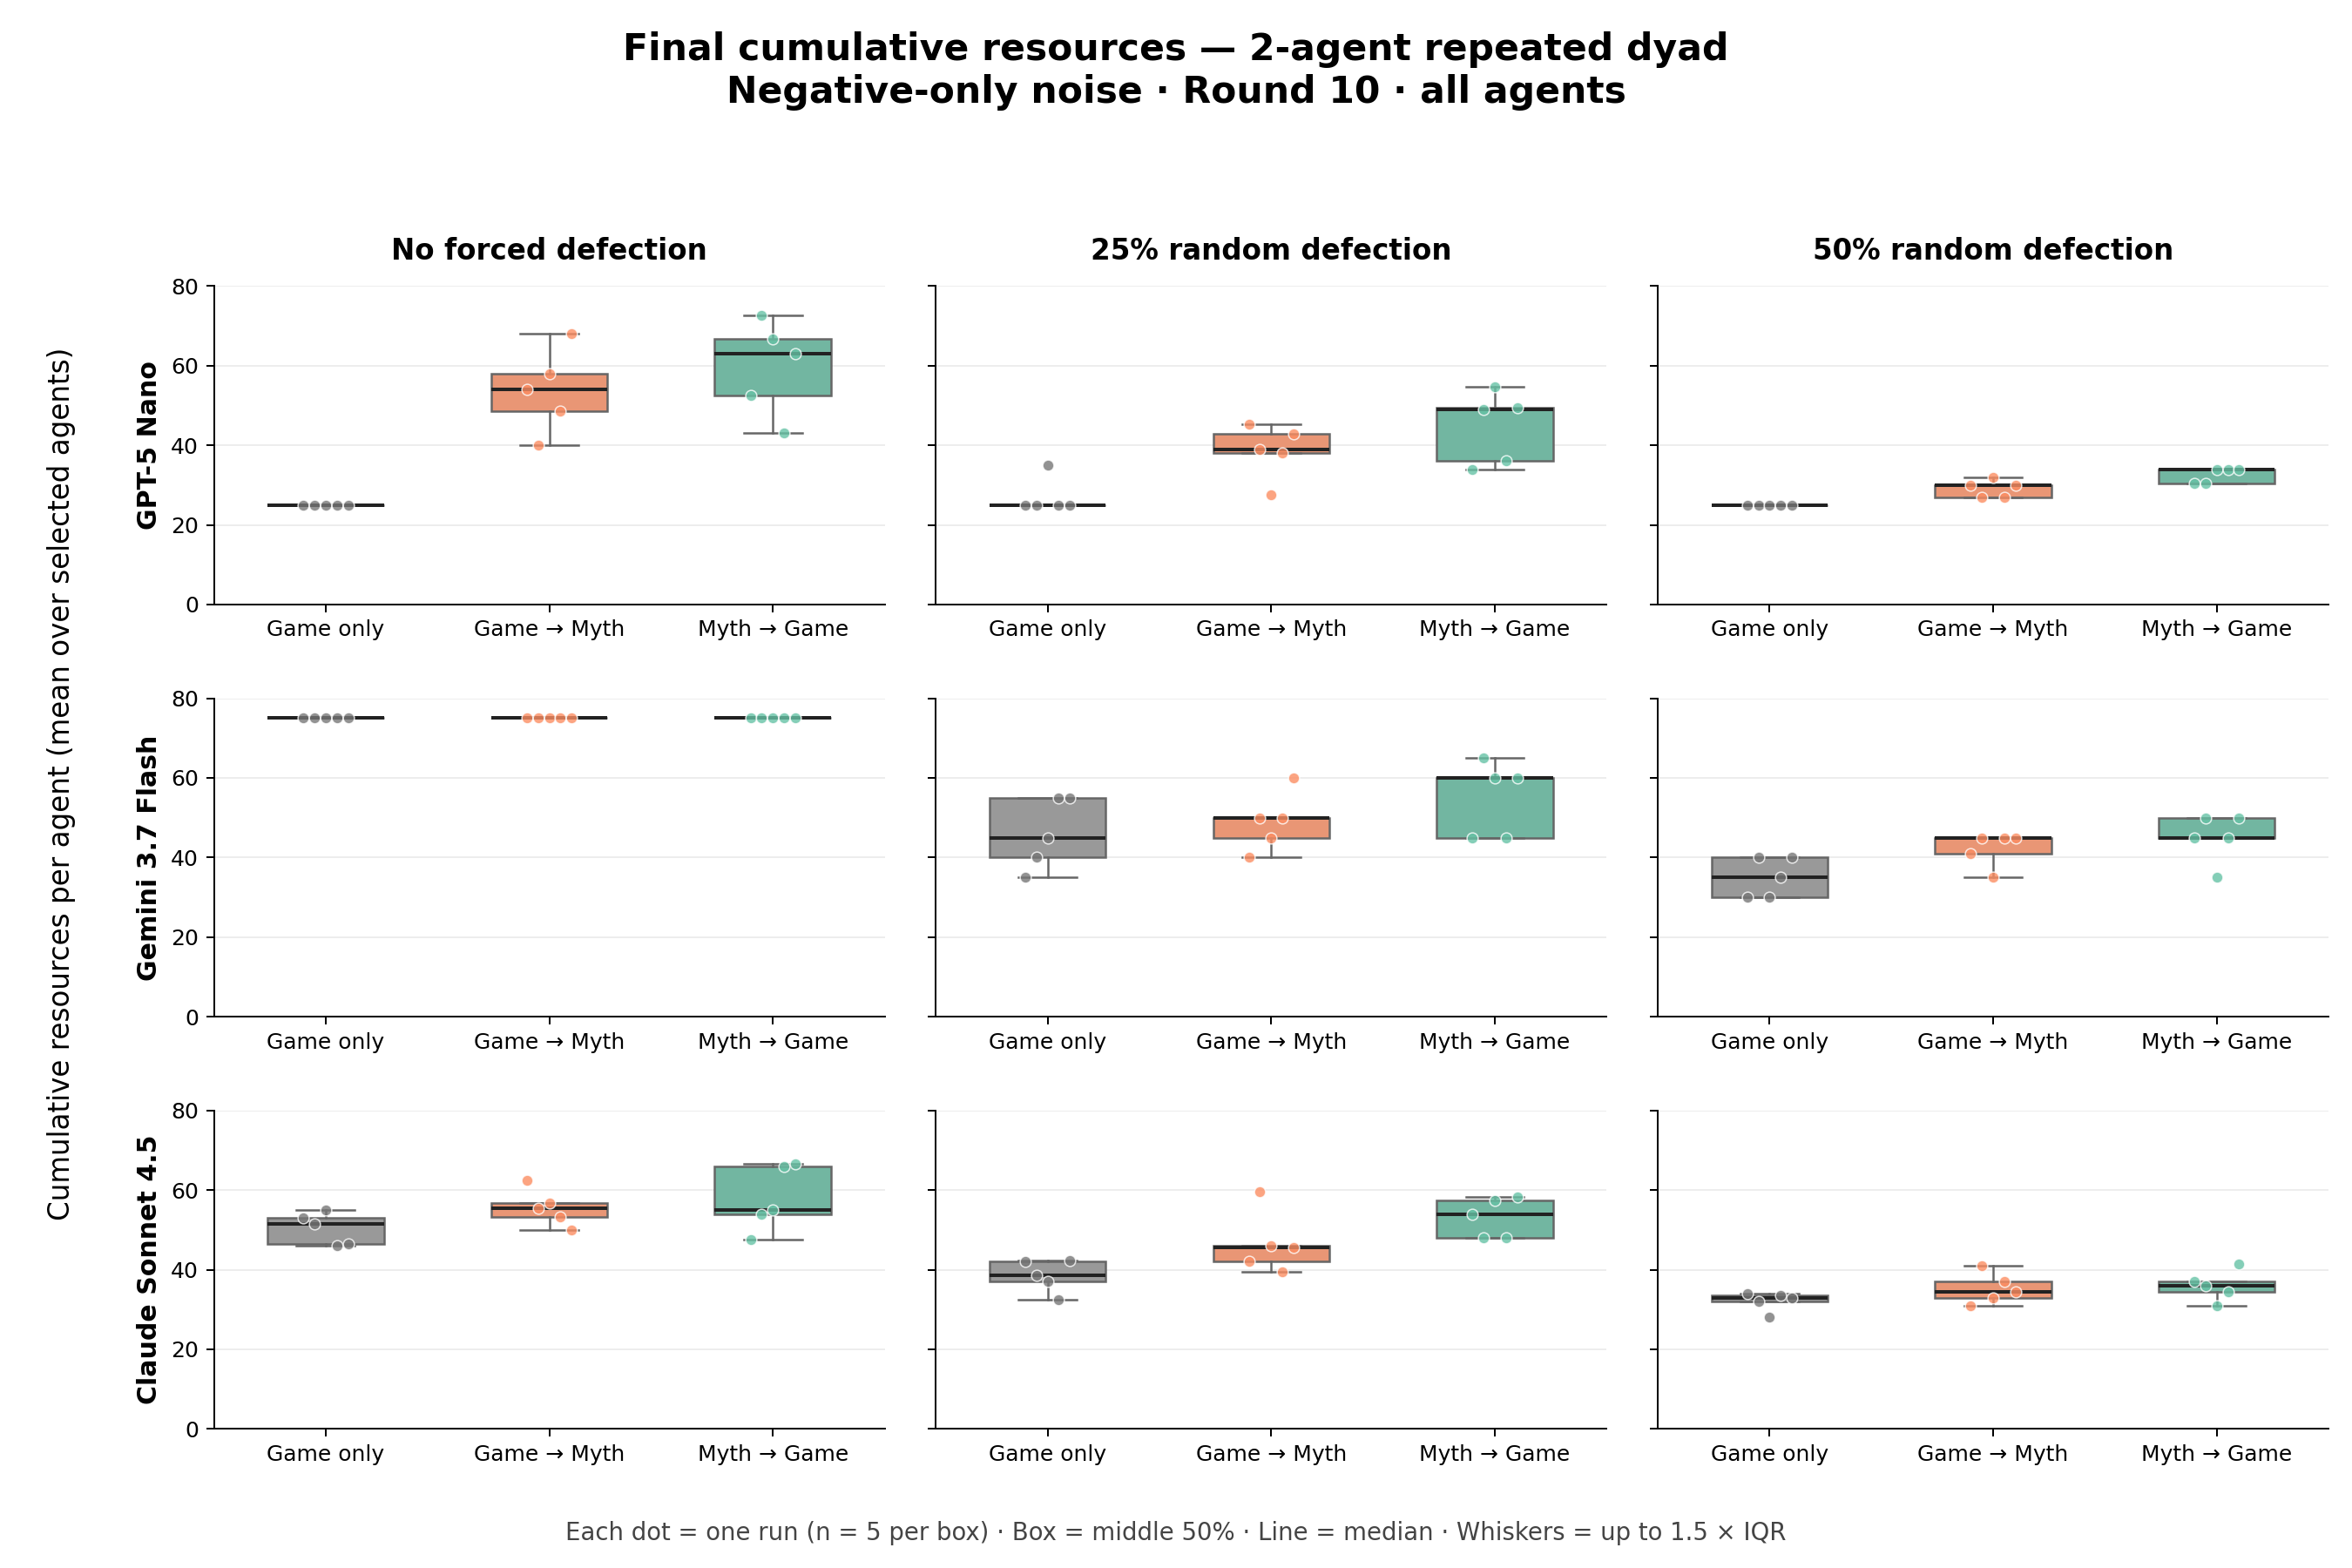
\includegraphics[width=\textwidth]{dyad_all_agents_boxplots.png}
  \caption{Two-agent repeated dyad: final cumulative resources under negative-only noise, averaged over all agents. Each dot represents one completed run after ten rounds (five runs per condition). Rows show models and columns show forced-defection conditions. Gray denotes Game only, orange Game $\rightarrow$ Myth, and teal Myth $\rightarrow$ Game. Boxes span the interquartile range, the central line marks the median, and whiskers extend to the most extreme observations within 1.5 interquartile ranges of the box. All runs, including outliers, are shown as dots.}
  \label{fig:dyad-resources-boxplots}
\end{figure*}

\begin{figure*}[tp]
  \centering
  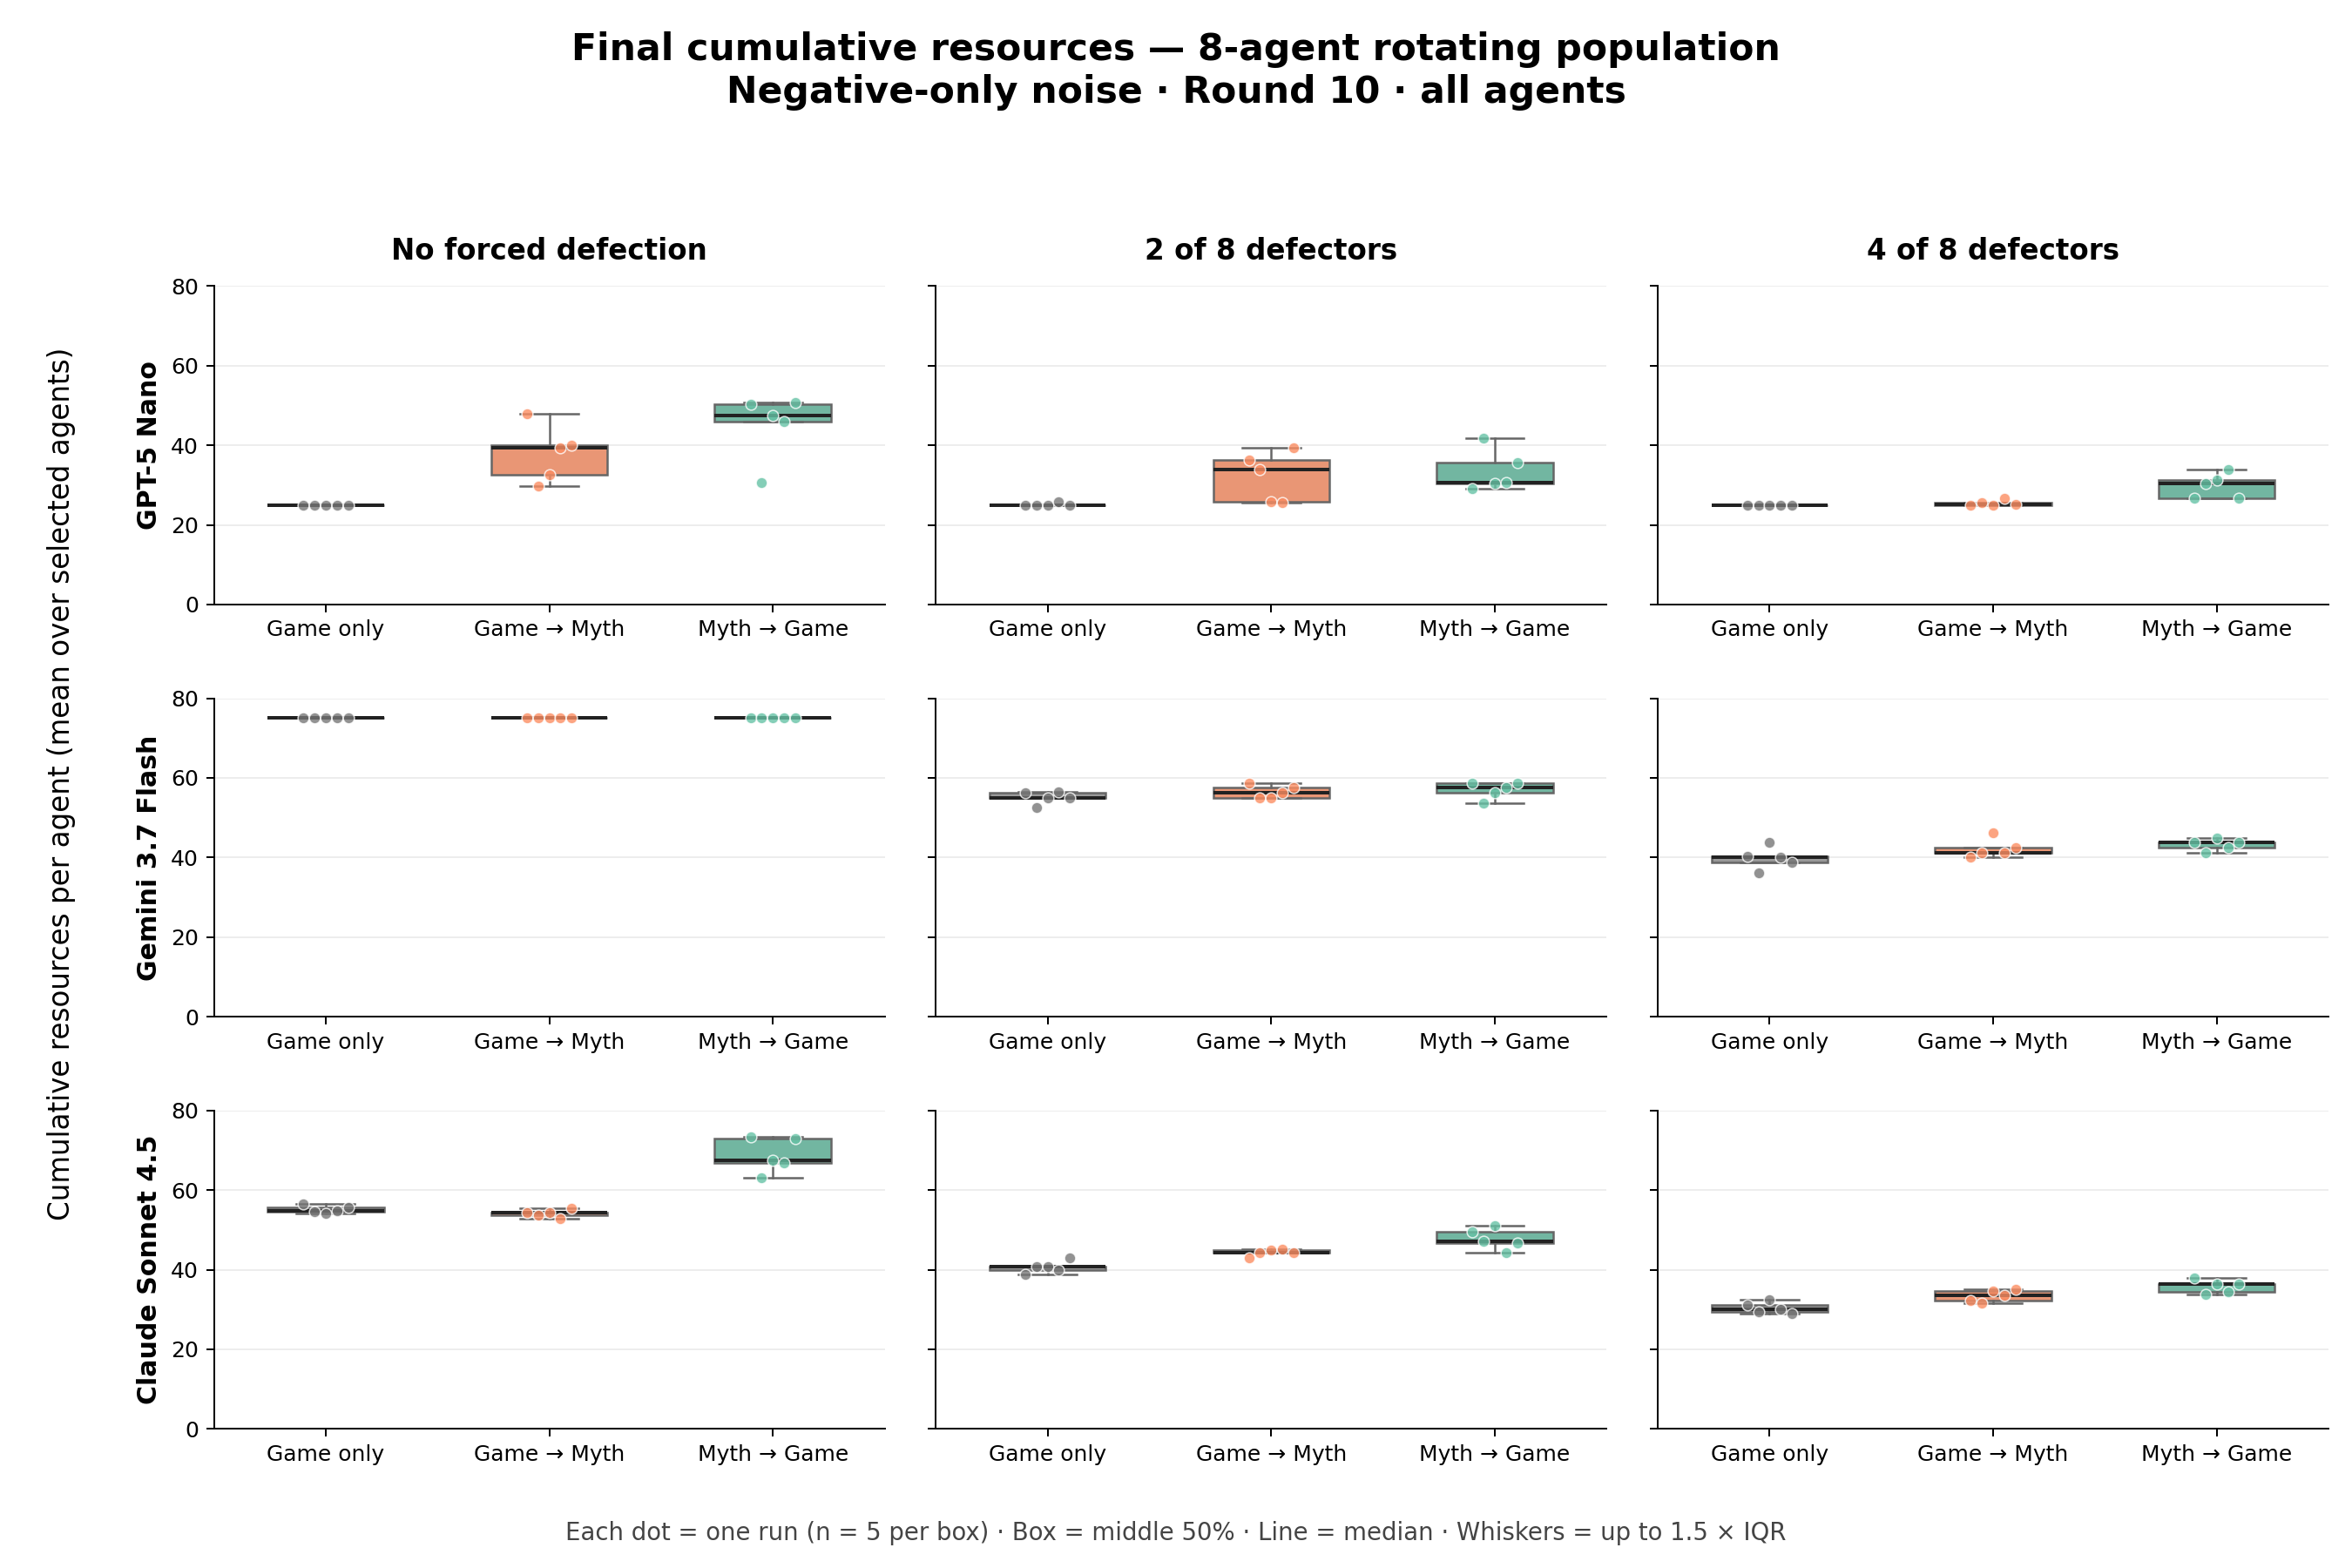
\includegraphics[width=\textwidth]{population_all_agents_boxplots.png}
  \caption{Eight-agent rotating population: final cumulative resources under negative-only noise, averaged over all agents. Each dot represents one completed run after ten rounds (five runs per condition). Rows show models and columns show forced-defection conditions. Gray denotes Game only, orange Game $\rightarrow$ Myth, and teal Myth $\rightarrow$ Game. Boxes span the interquartile range, the central line marks the median, and whiskers extend to the most extreme observations within 1.5 interquartile ranges of the box. All runs, including outliers, are shown as dots.}
  \label{fig:population-resources-boxplots}
\end{figure*}

\begin{figure*}[tp]
  \centering
  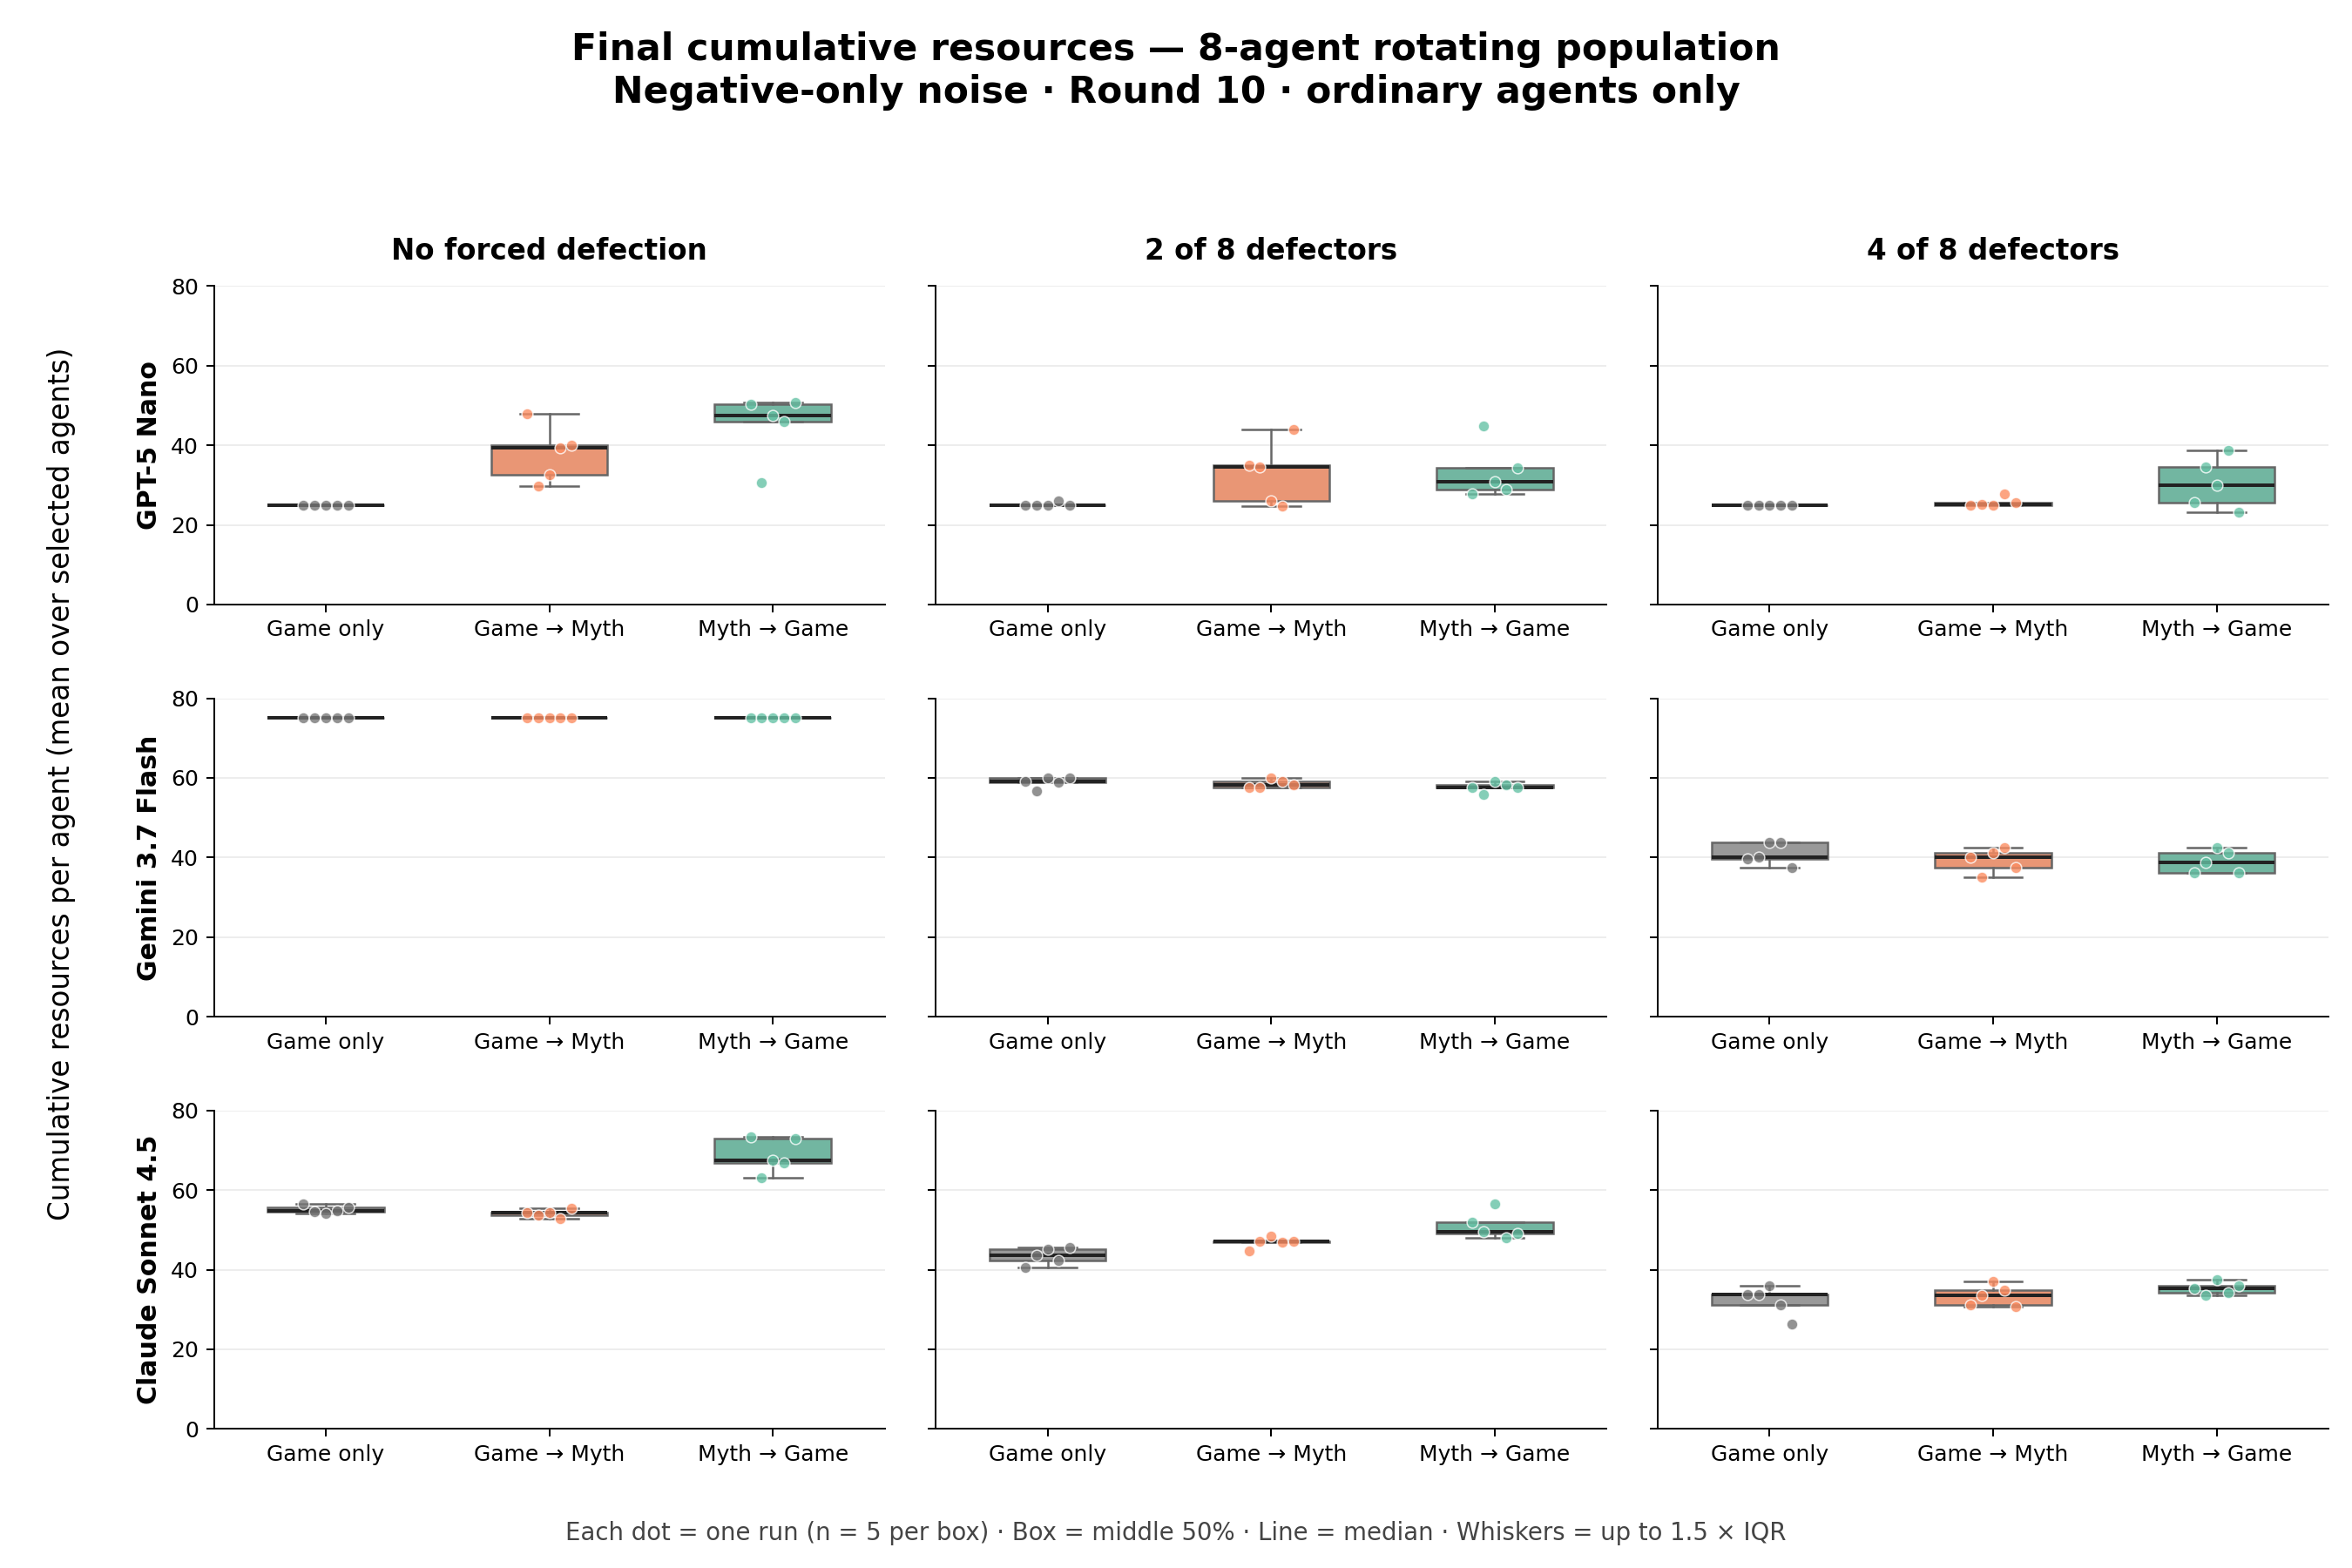
\includegraphics[width=\textwidth]{population_ordinary_agents_boxplots.png}
  \caption{Eight-agent rotating population: final cumulative resources under negative-only noise, averaged over ordinary (non-defector) agents only. Each dot represents one completed run after ten rounds (five runs per condition). Rows show models and columns show forced-defection conditions. Gray denotes Game only, orange Game $\rightarrow$ Myth, and teal Myth $\rightarrow$ Game. Boxes span the interquartile range, the central line marks the median, and whiskers extend to the most extreme observations within 1.5 interquartile ranges of the box. All runs, including outliers, are shown as dots.}
  \label{fig:ordinary-resources-boxplots}
\end{figure*}
 inside the Results section.

\begin{figure*}[tp]
  \centering
  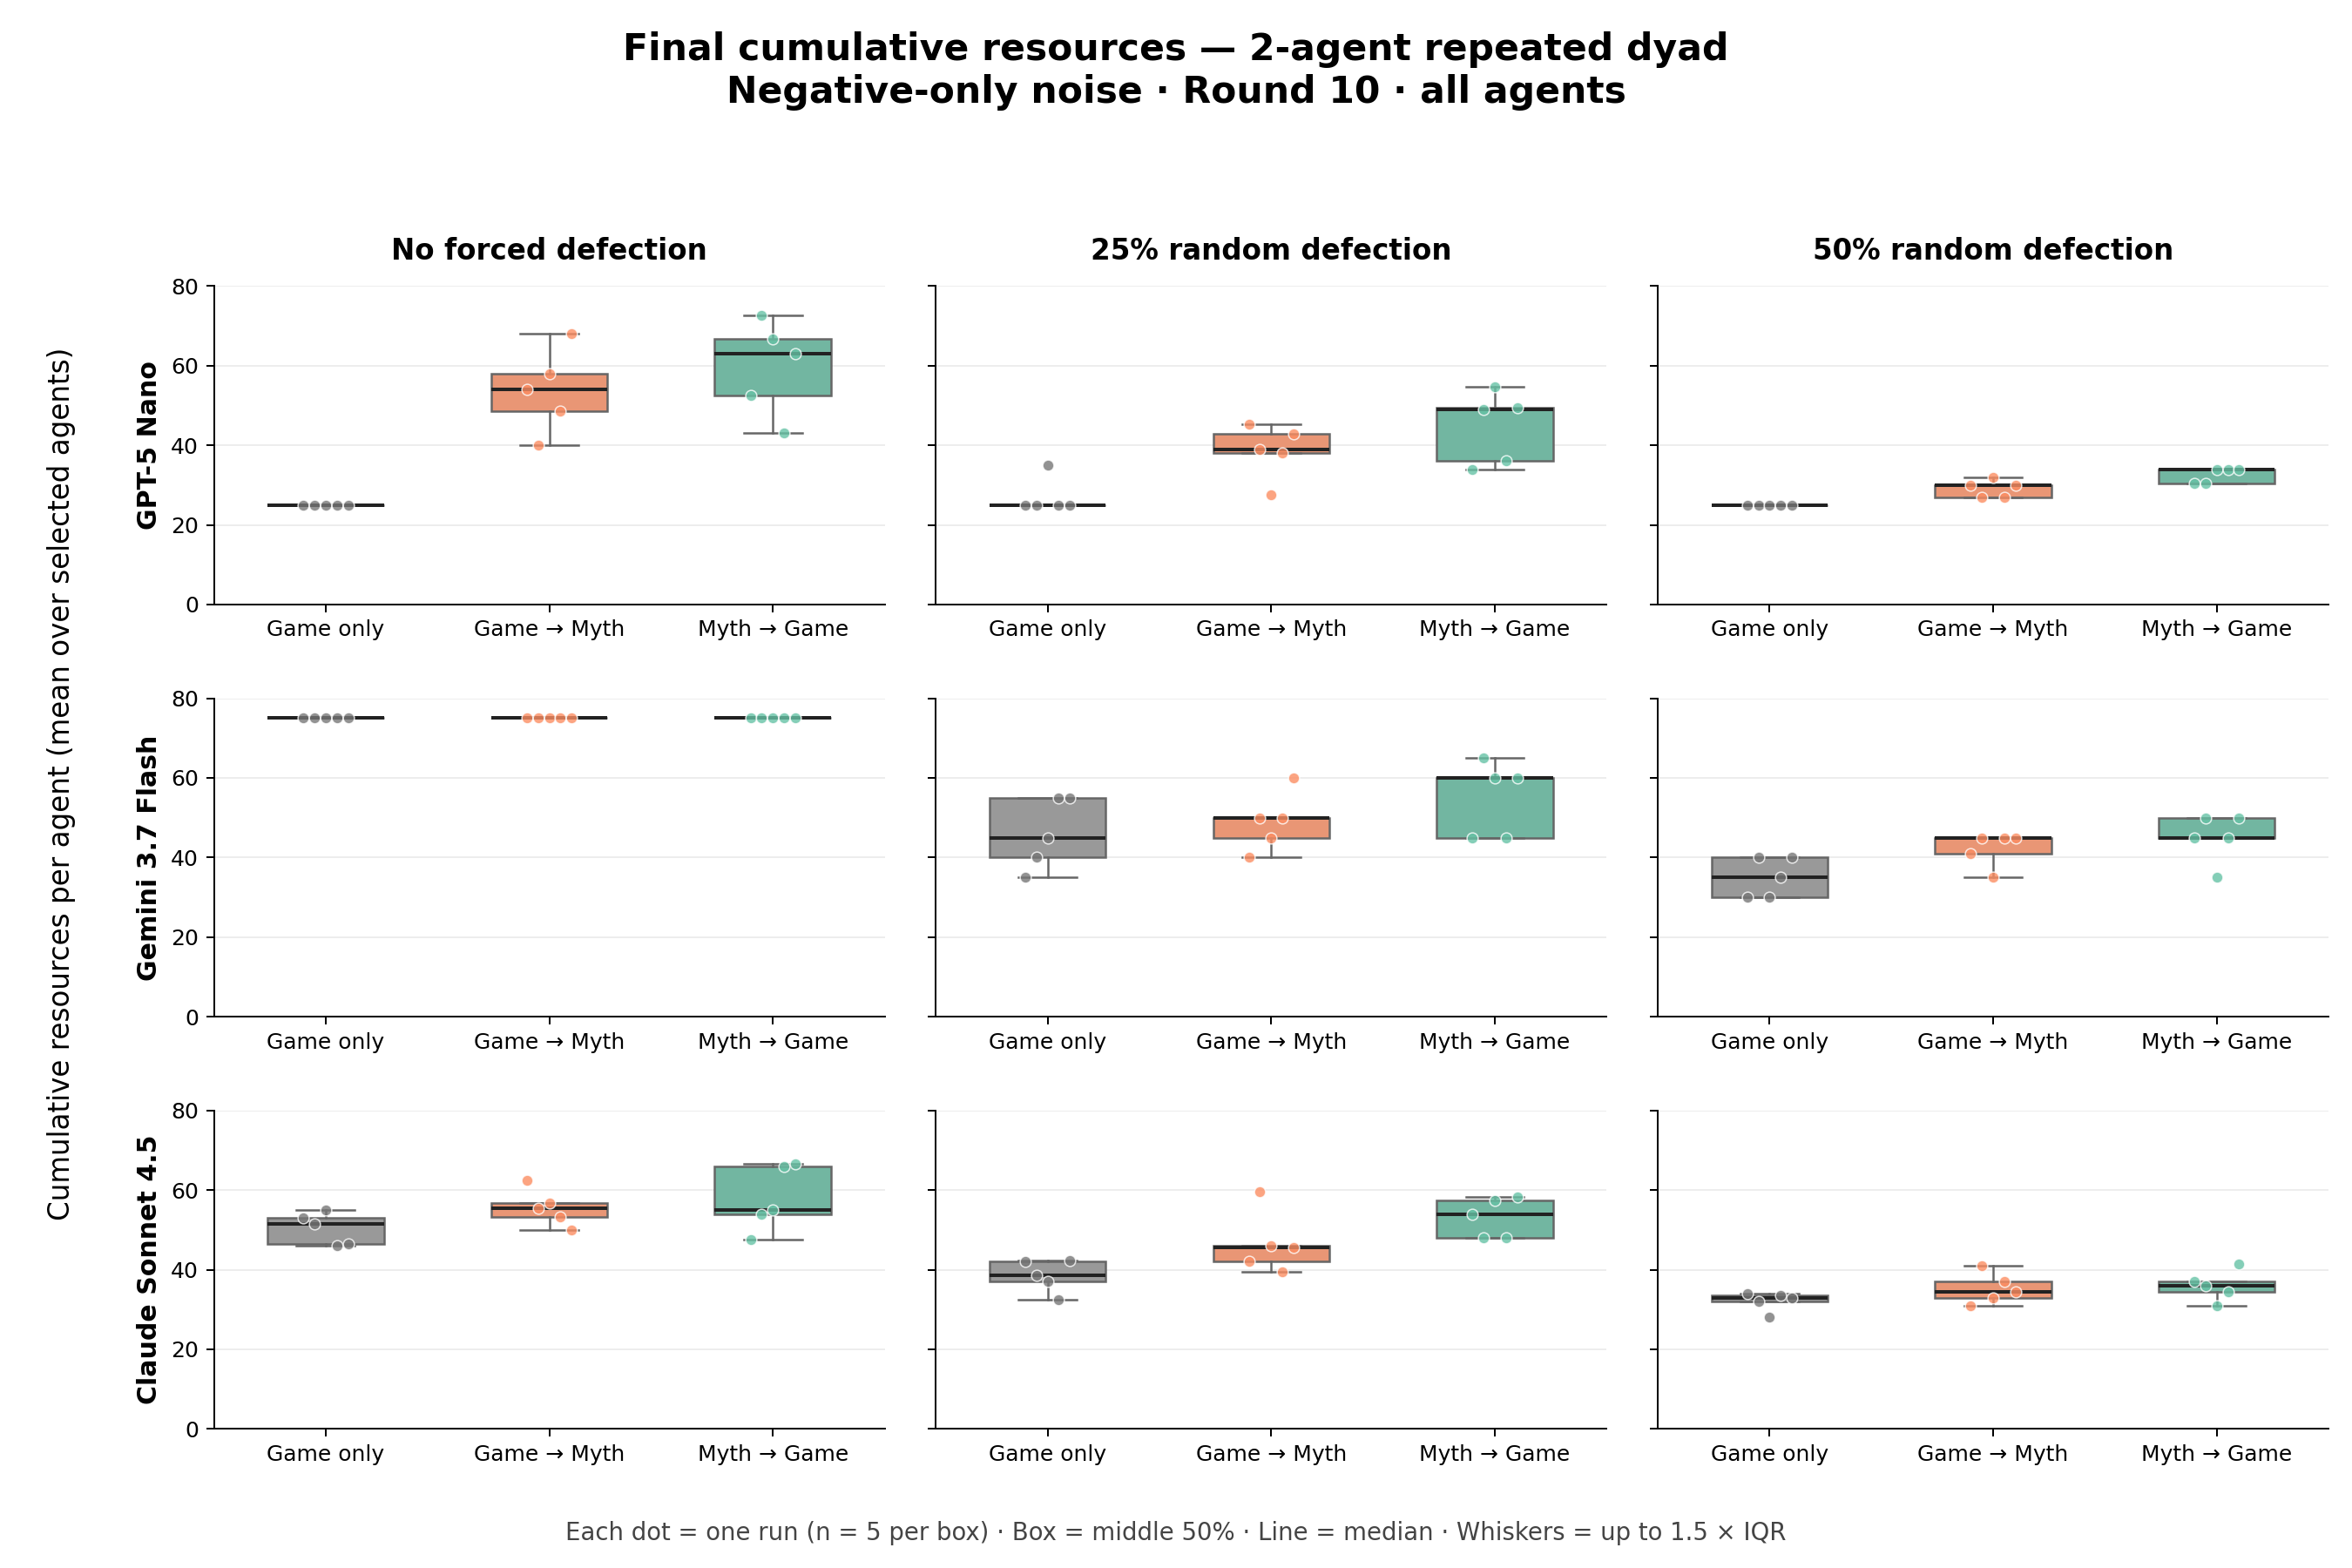
\includegraphics[width=\textwidth]{dyad_all_agents_boxplots.png}
  \caption{Two-agent repeated dyad: final cumulative resources under negative-only noise, averaged over all agents. Each dot represents one completed run after ten rounds (five runs per condition). Rows show models and columns show forced-defection conditions. Gray denotes Game only, orange Game $\rightarrow$ Myth, and teal Myth $\rightarrow$ Game. Boxes span the interquartile range, the central line marks the median, and whiskers extend to the most extreme observations within 1.5 interquartile ranges of the box. All runs, including outliers, are shown as dots.}
  \label{fig:dyad-resources-boxplots}
\end{figure*}

\begin{figure*}[tp]
  \centering
  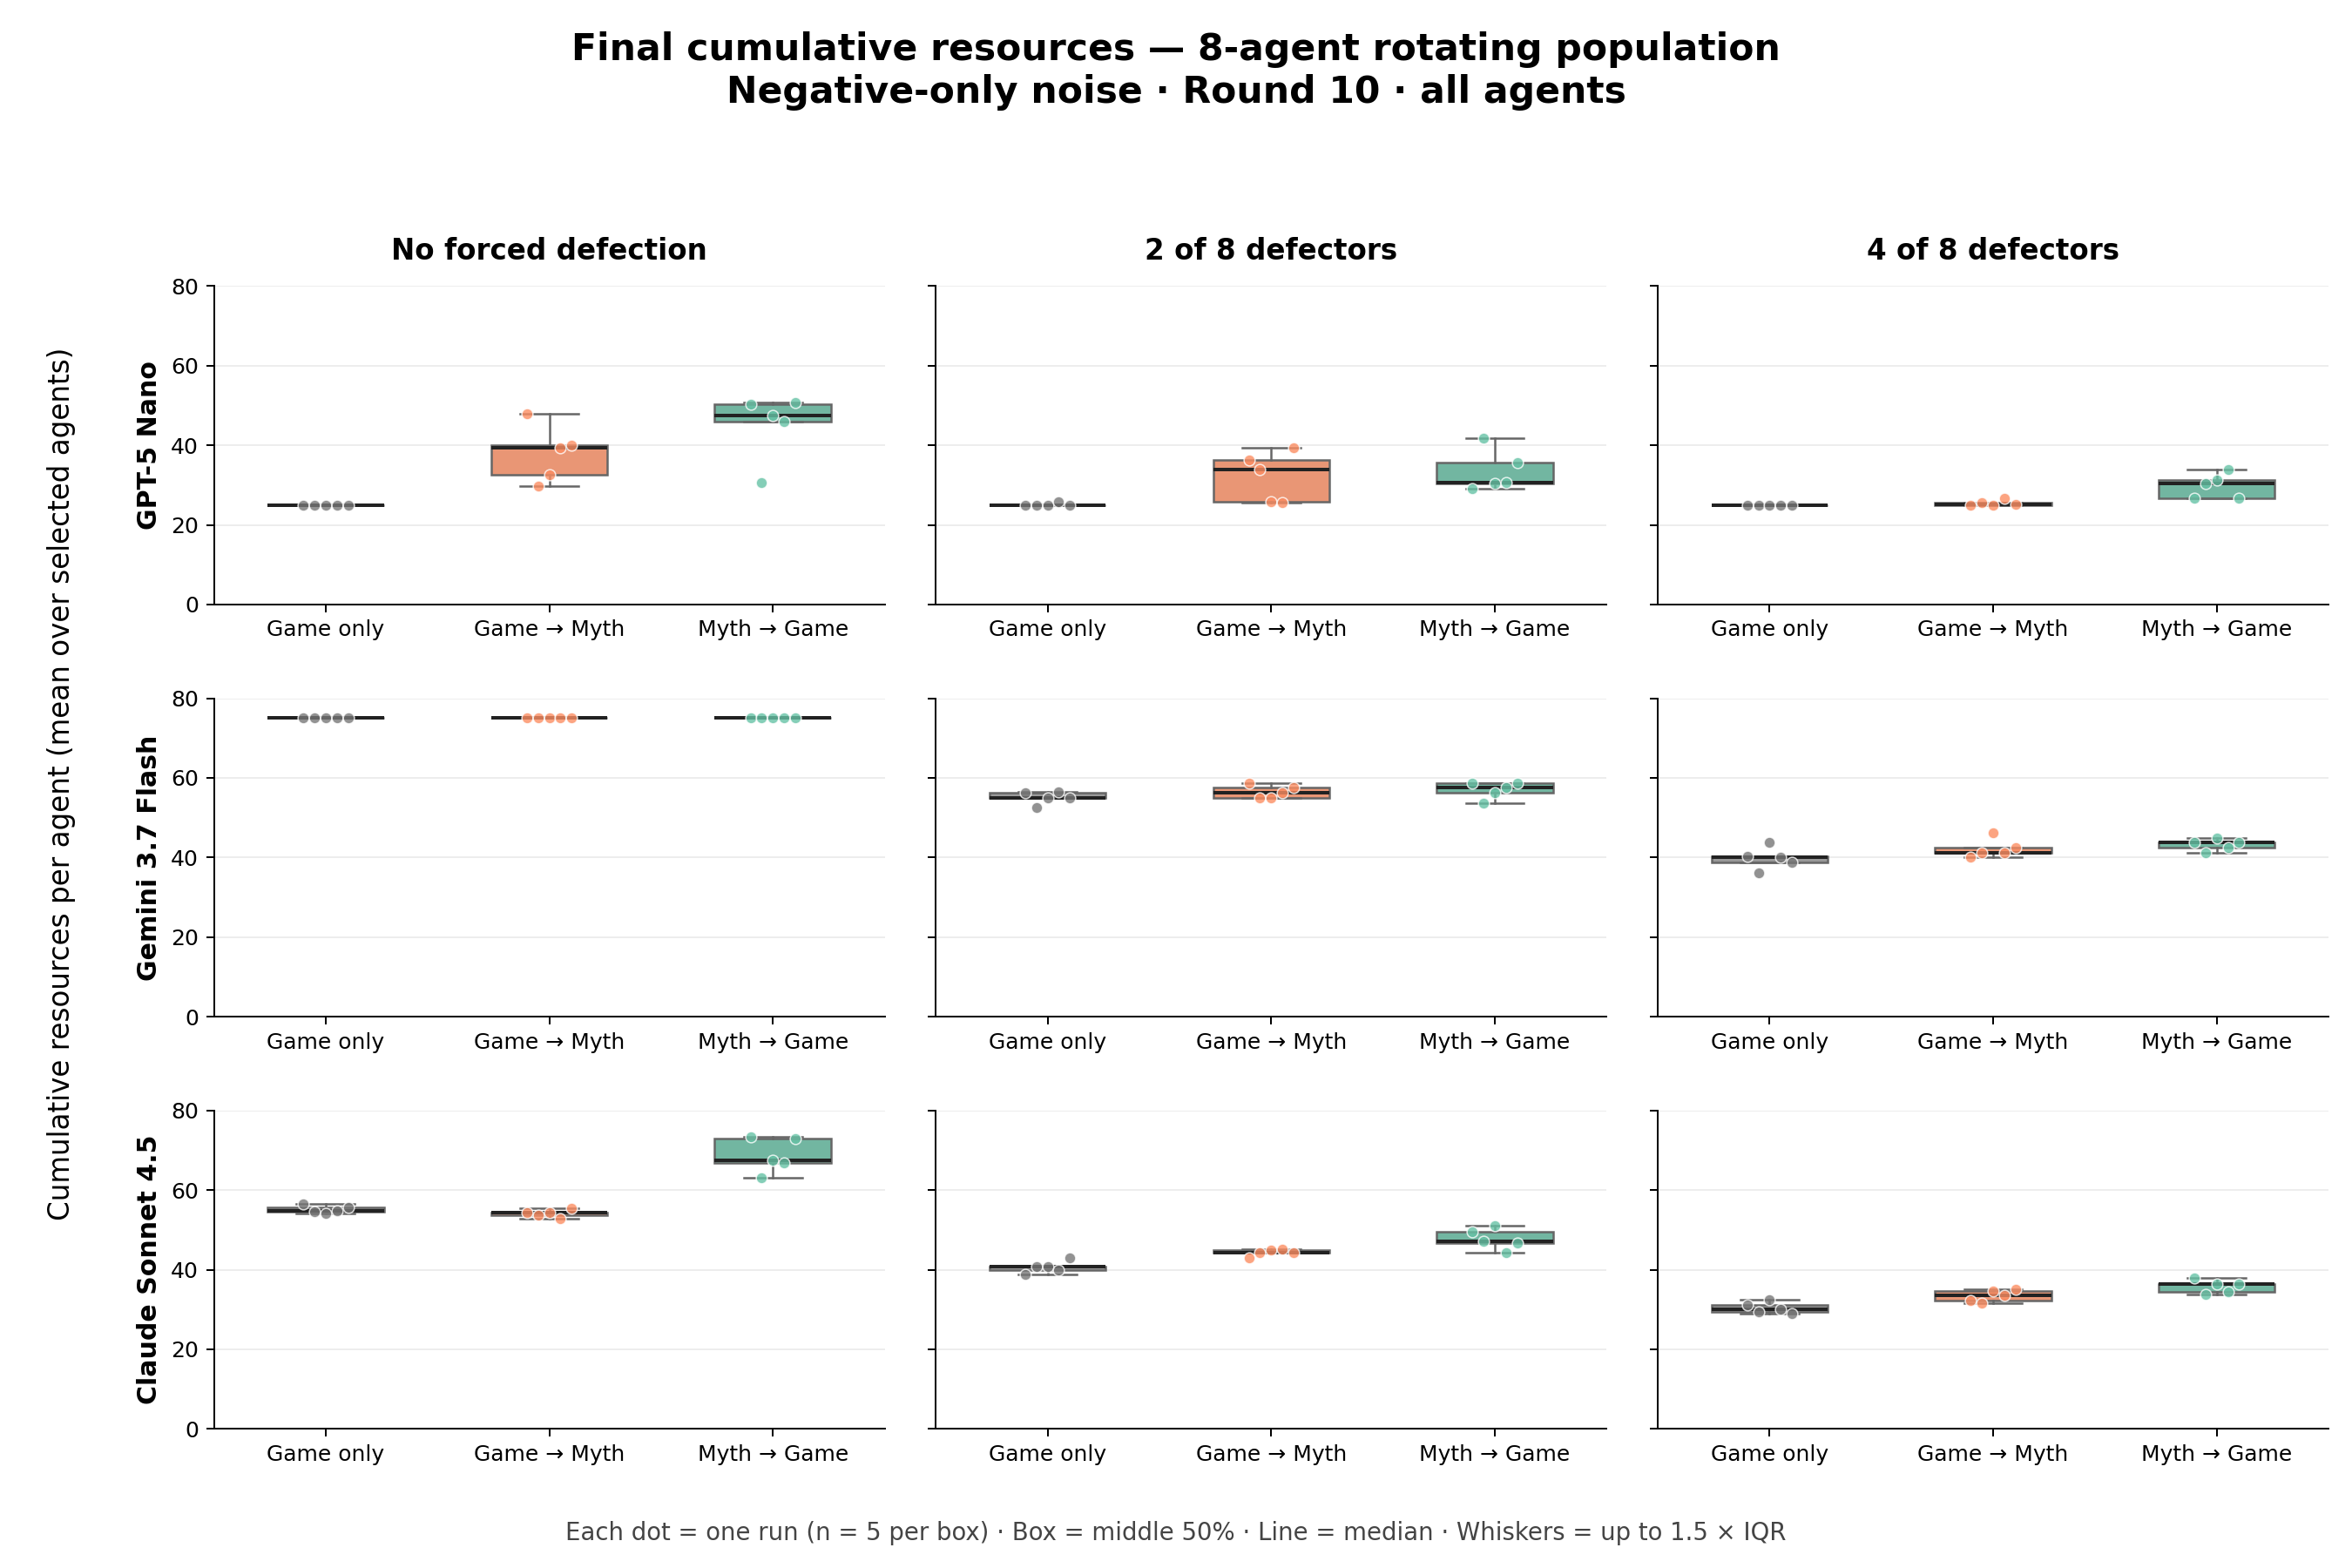
\includegraphics[width=\textwidth]{population_all_agents_boxplots.png}
  \caption{Eight-agent rotating population: final cumulative resources under negative-only noise, averaged over all agents. Each dot represents one completed run after ten rounds (five runs per condition). Rows show models and columns show forced-defection conditions. Gray denotes Game only, orange Game $\rightarrow$ Myth, and teal Myth $\rightarrow$ Game. Boxes span the interquartile range, the central line marks the median, and whiskers extend to the most extreme observations within 1.5 interquartile ranges of the box. All runs, including outliers, are shown as dots.}
  \label{fig:population-resources-boxplots}
\end{figure*}

\begin{figure*}[tp]
  \centering
  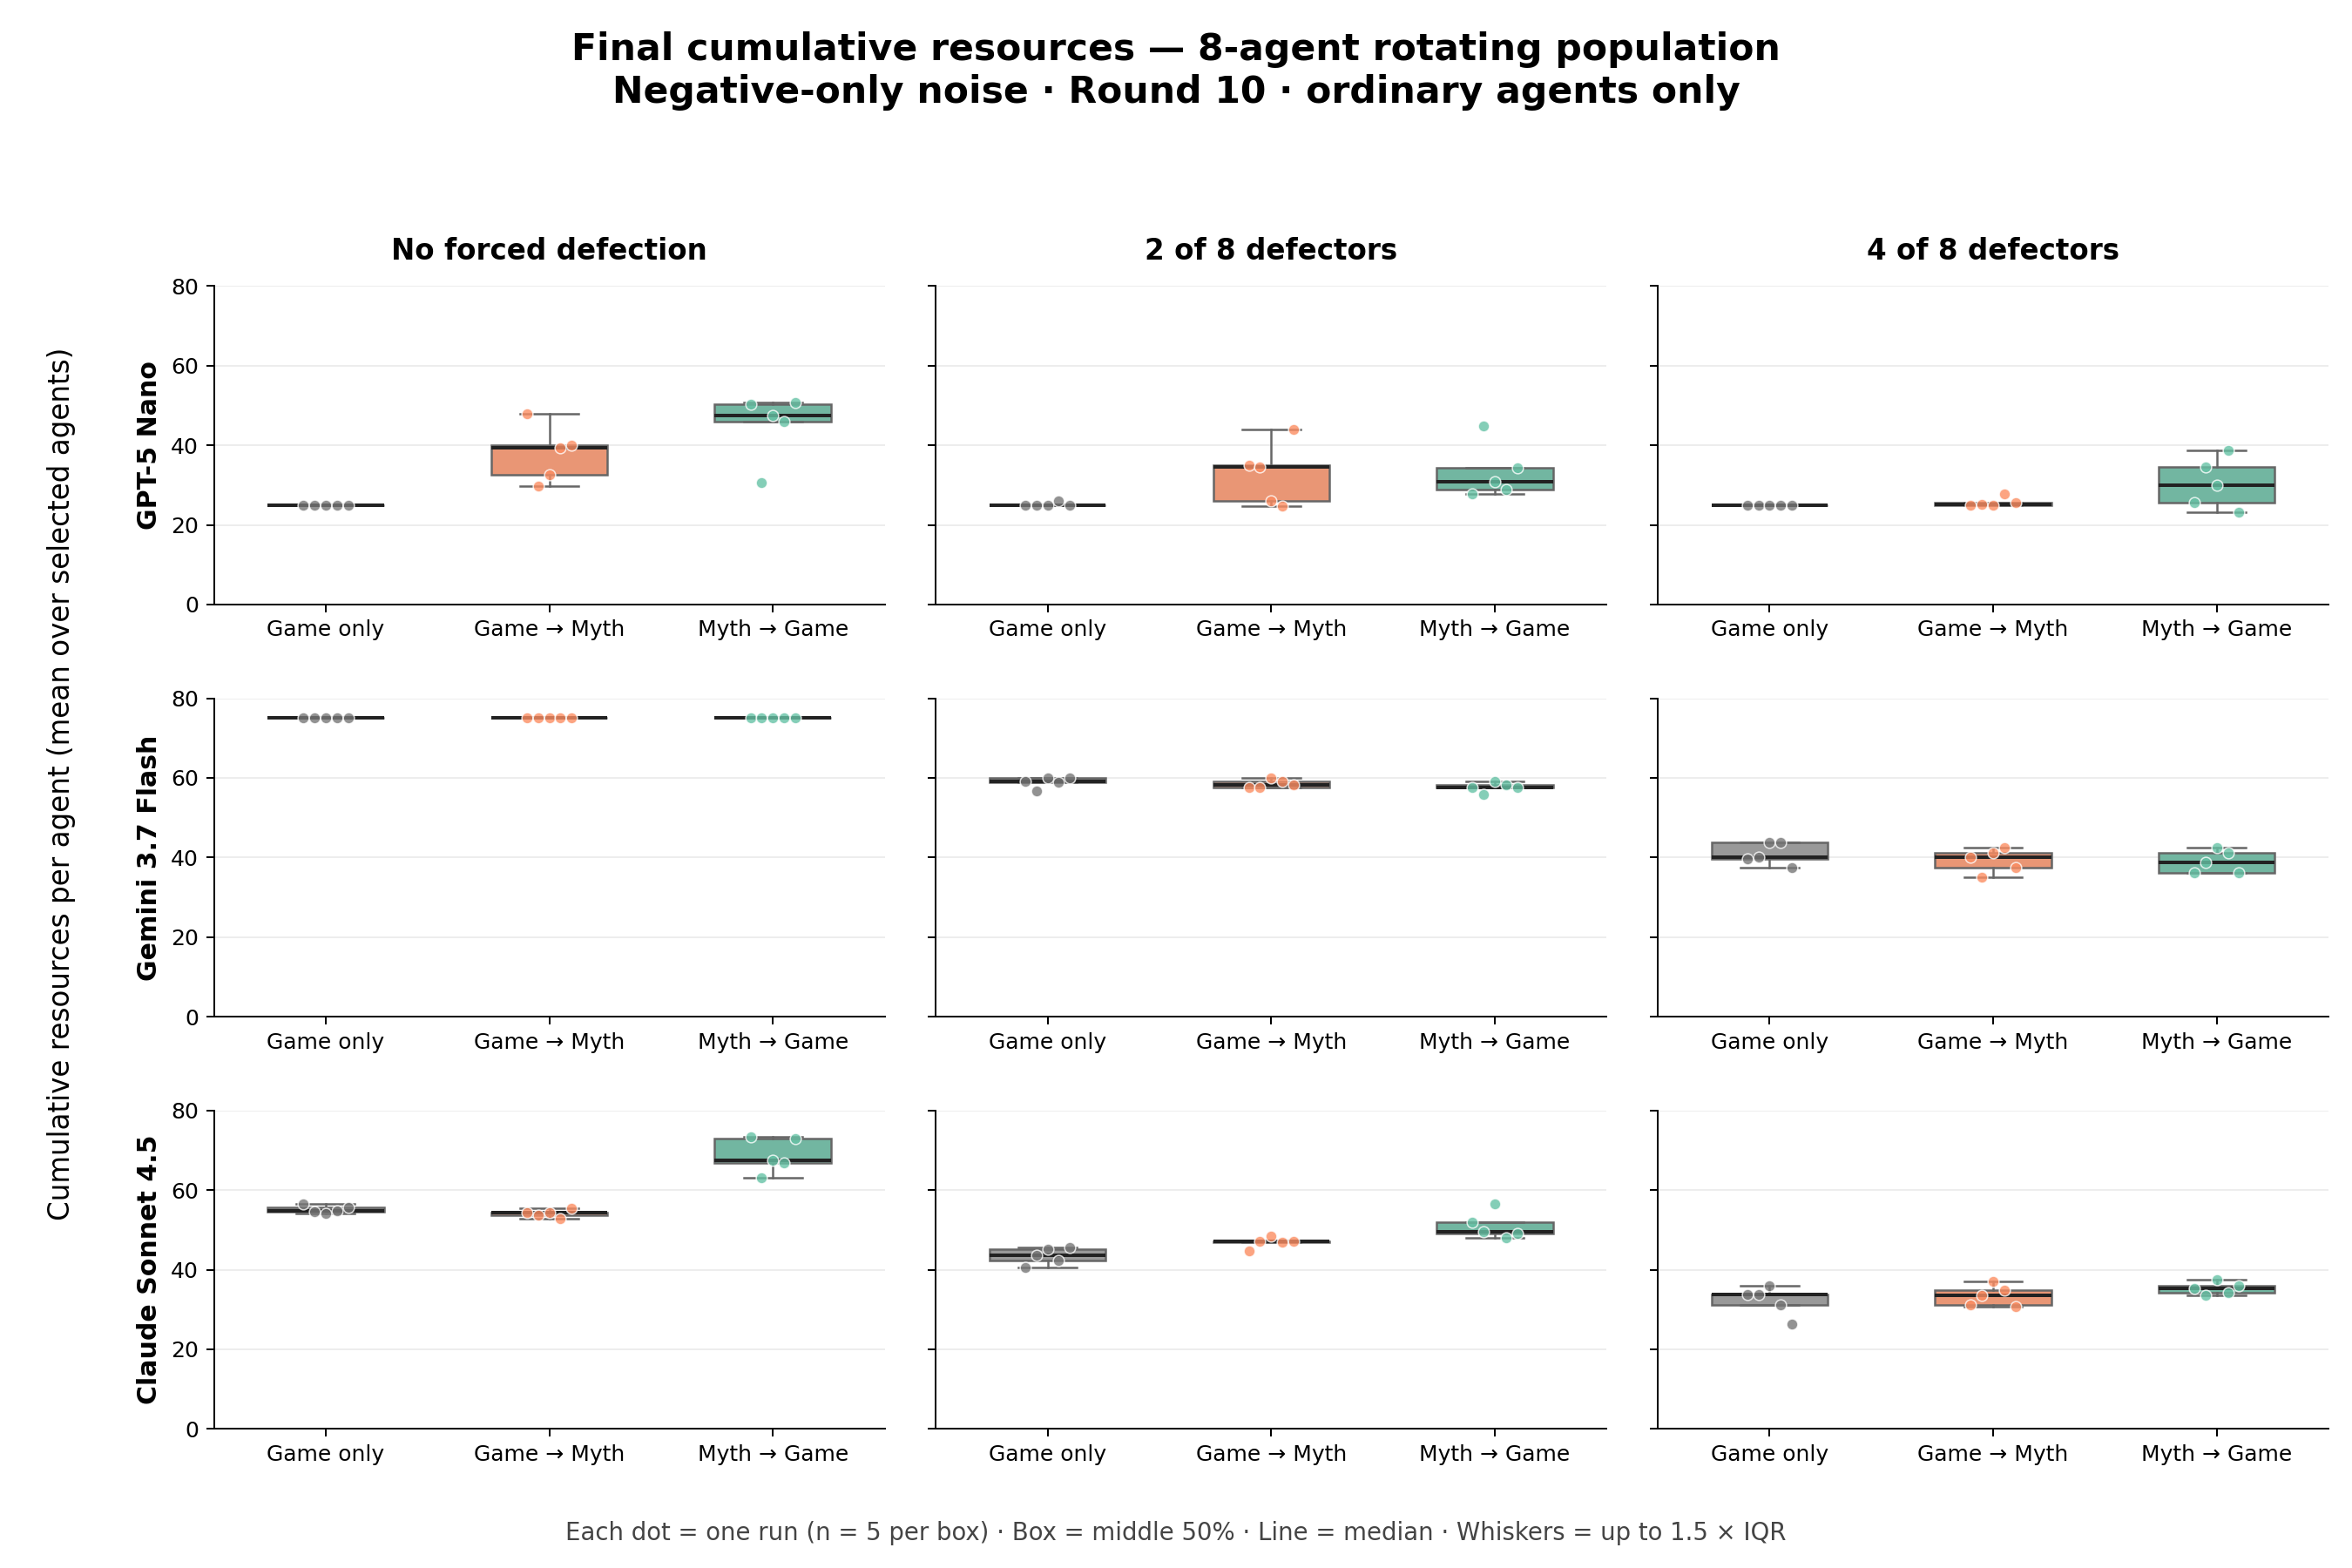
\includegraphics[width=\textwidth]{population_ordinary_agents_boxplots.png}
  \caption{Eight-agent rotating population: final cumulative resources under negative-only noise, averaged over ordinary (non-defector) agents only. Each dot represents one completed run after ten rounds (five runs per condition). Rows show models and columns show forced-defection conditions. Gray denotes Game only, orange Game $\rightarrow$ Myth, and teal Myth $\rightarrow$ Game. Boxes span the interquartile range, the central line marks the median, and whiskers extend to the most extreme observations within 1.5 interquartile ranges of the box. All runs, including outliers, are shown as dots.}
  \label{fig:ordinary-resources-boxplots}
\end{figure*}
 inside the Results section.

\begin{figure*}[tp]
  \centering
  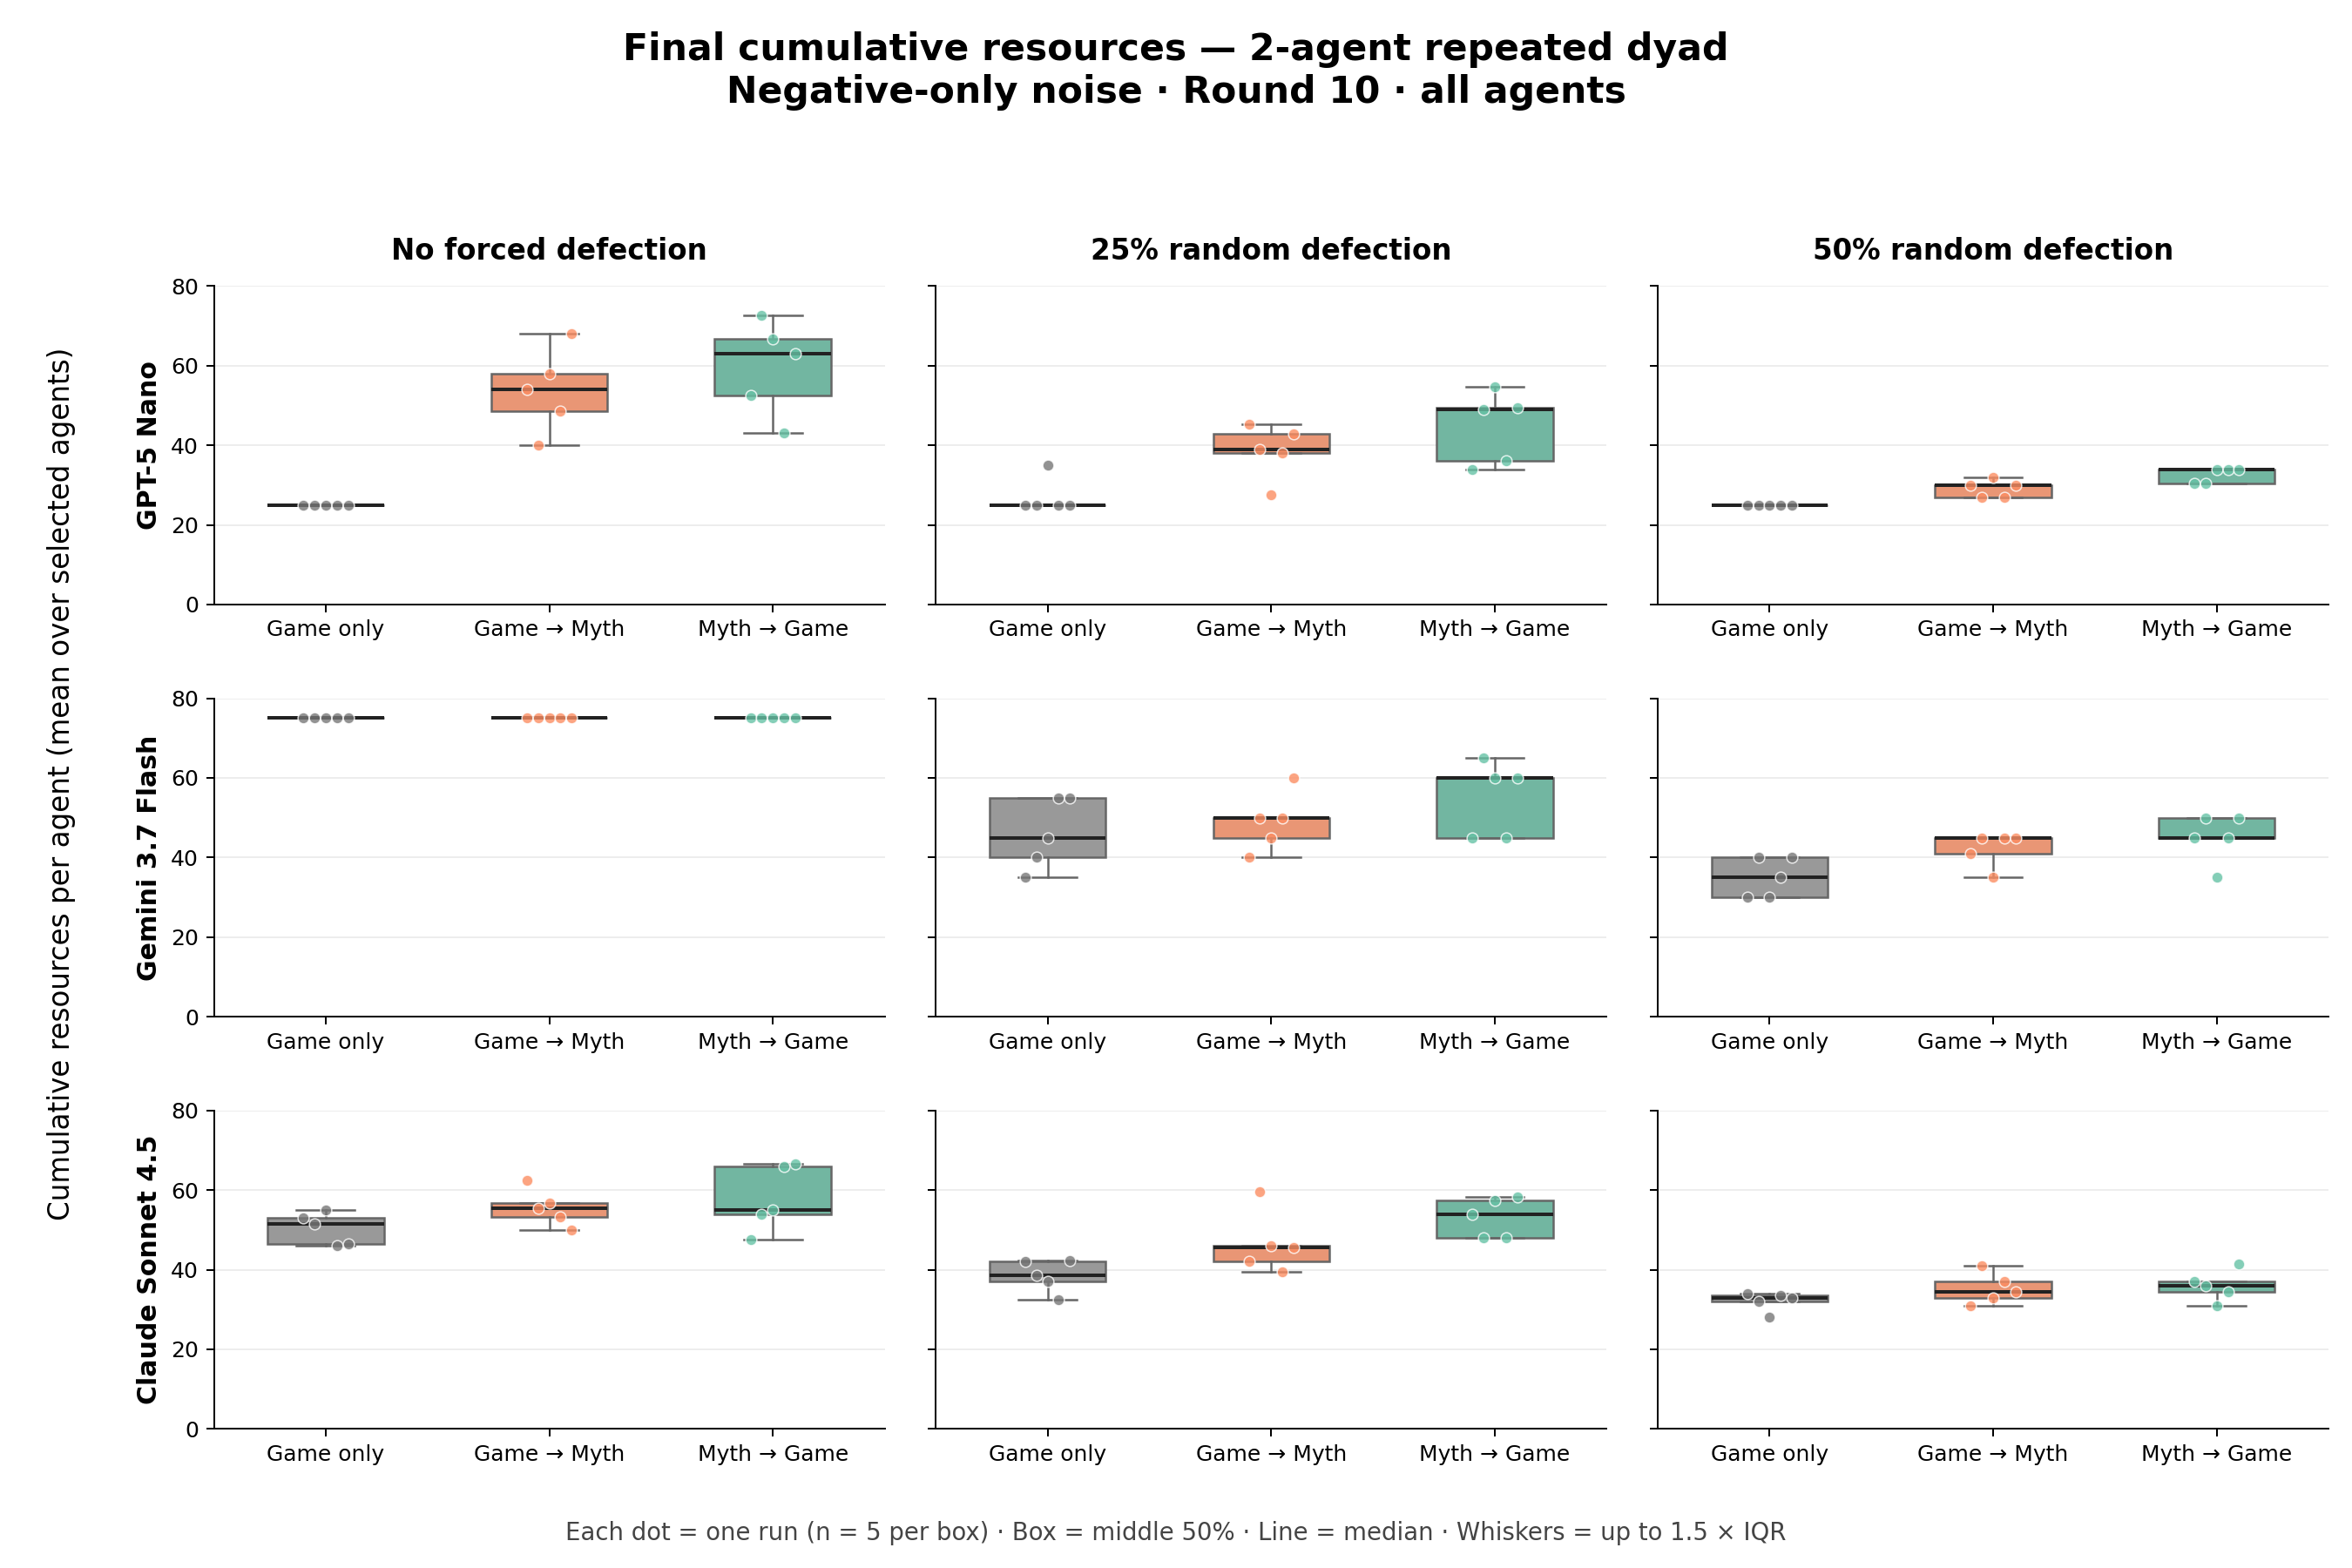
\includegraphics[width=\textwidth]{dyad_all_agents_boxplots.png}
  \caption{Two-agent repeated dyad: final cumulative resources under negative-only noise, averaged over all agents. Each dot represents one completed run after ten rounds (five runs per condition). Rows show models and columns show forced-defection conditions. Gray denotes Game only, orange Game $\rightarrow$ Myth, and teal Myth $\rightarrow$ Game. Boxes span the interquartile range, the central line marks the median, and whiskers extend to the most extreme observations within 1.5 interquartile ranges of the box. All runs, including outliers, are shown as dots.}
  \label{fig:dyad-resources-boxplots}
\end{figure*}

\begin{figure*}[tp]
  \centering
  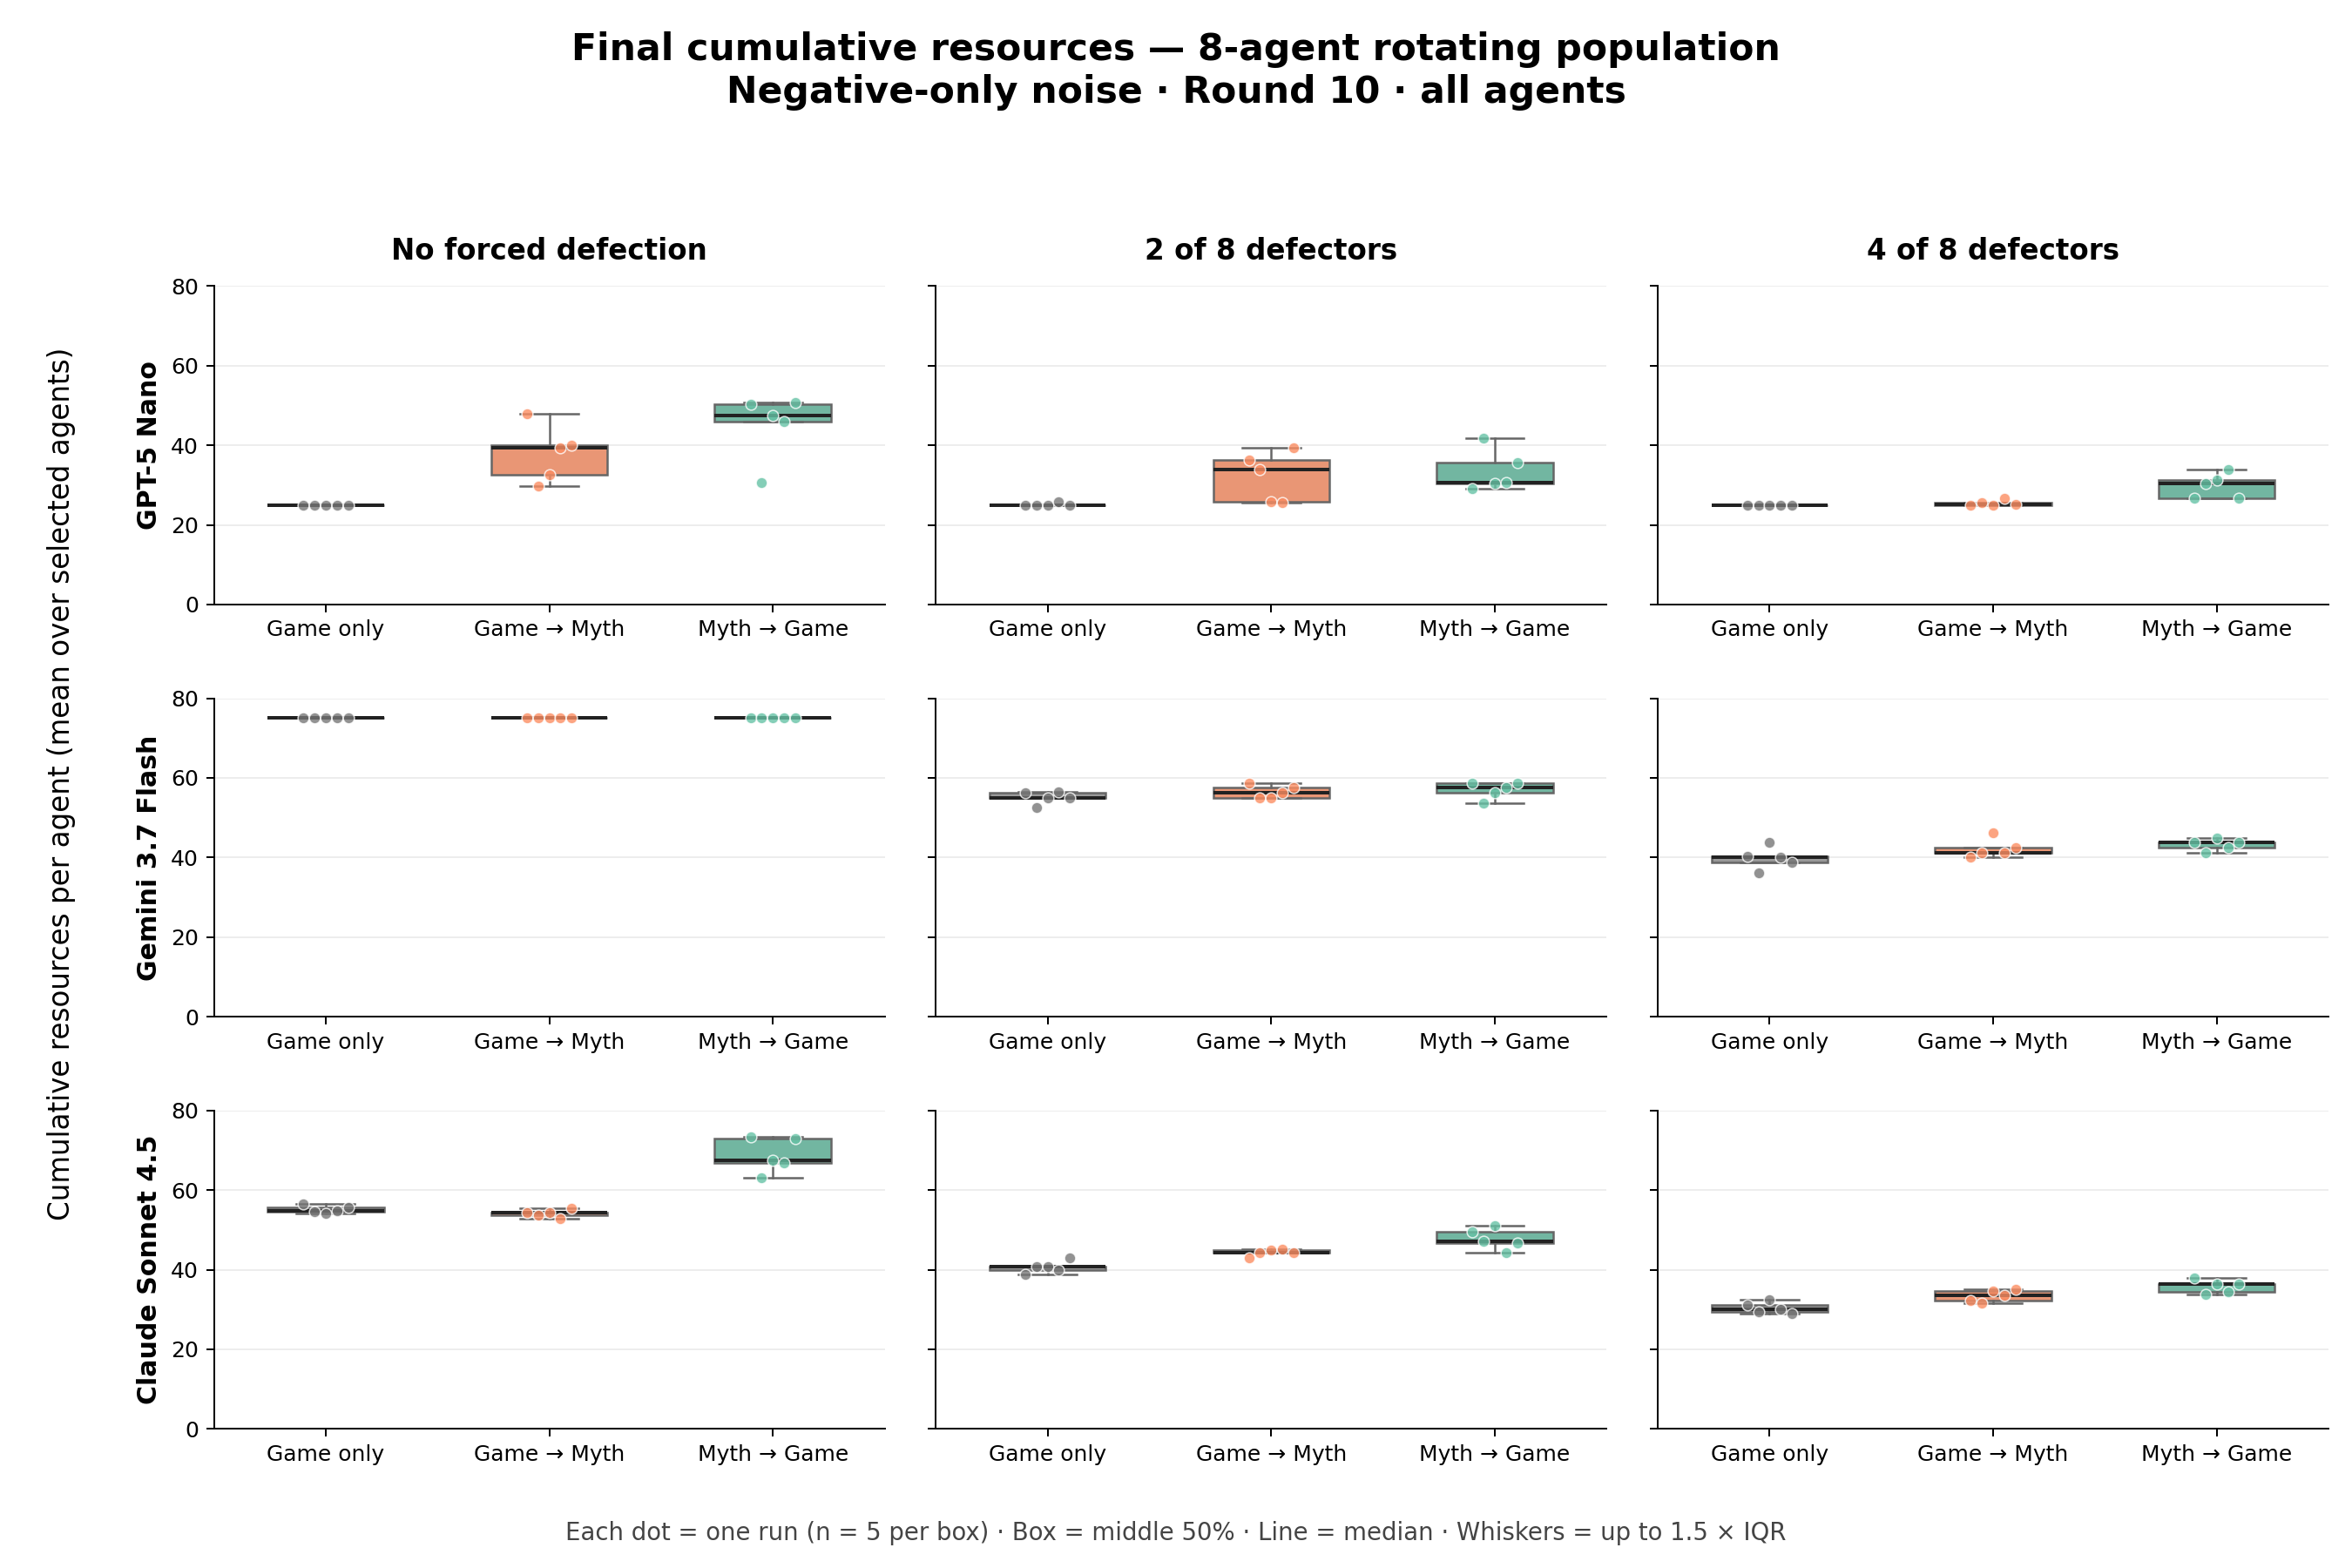
\includegraphics[width=\textwidth]{population_all_agents_boxplots.png}
  \caption{Eight-agent rotating population: final cumulative resources under negative-only noise, averaged over all agents. Each dot represents one completed run after ten rounds (five runs per condition). Rows show models and columns show forced-defection conditions. Gray denotes Game only, orange Game $\rightarrow$ Myth, and teal Myth $\rightarrow$ Game. Boxes span the interquartile range, the central line marks the median, and whiskers extend to the most extreme observations within 1.5 interquartile ranges of the box. All runs, including outliers, are shown as dots.}
  \label{fig:population-resources-boxplots}
\end{figure*}

\begin{figure*}[tp]
  \centering
  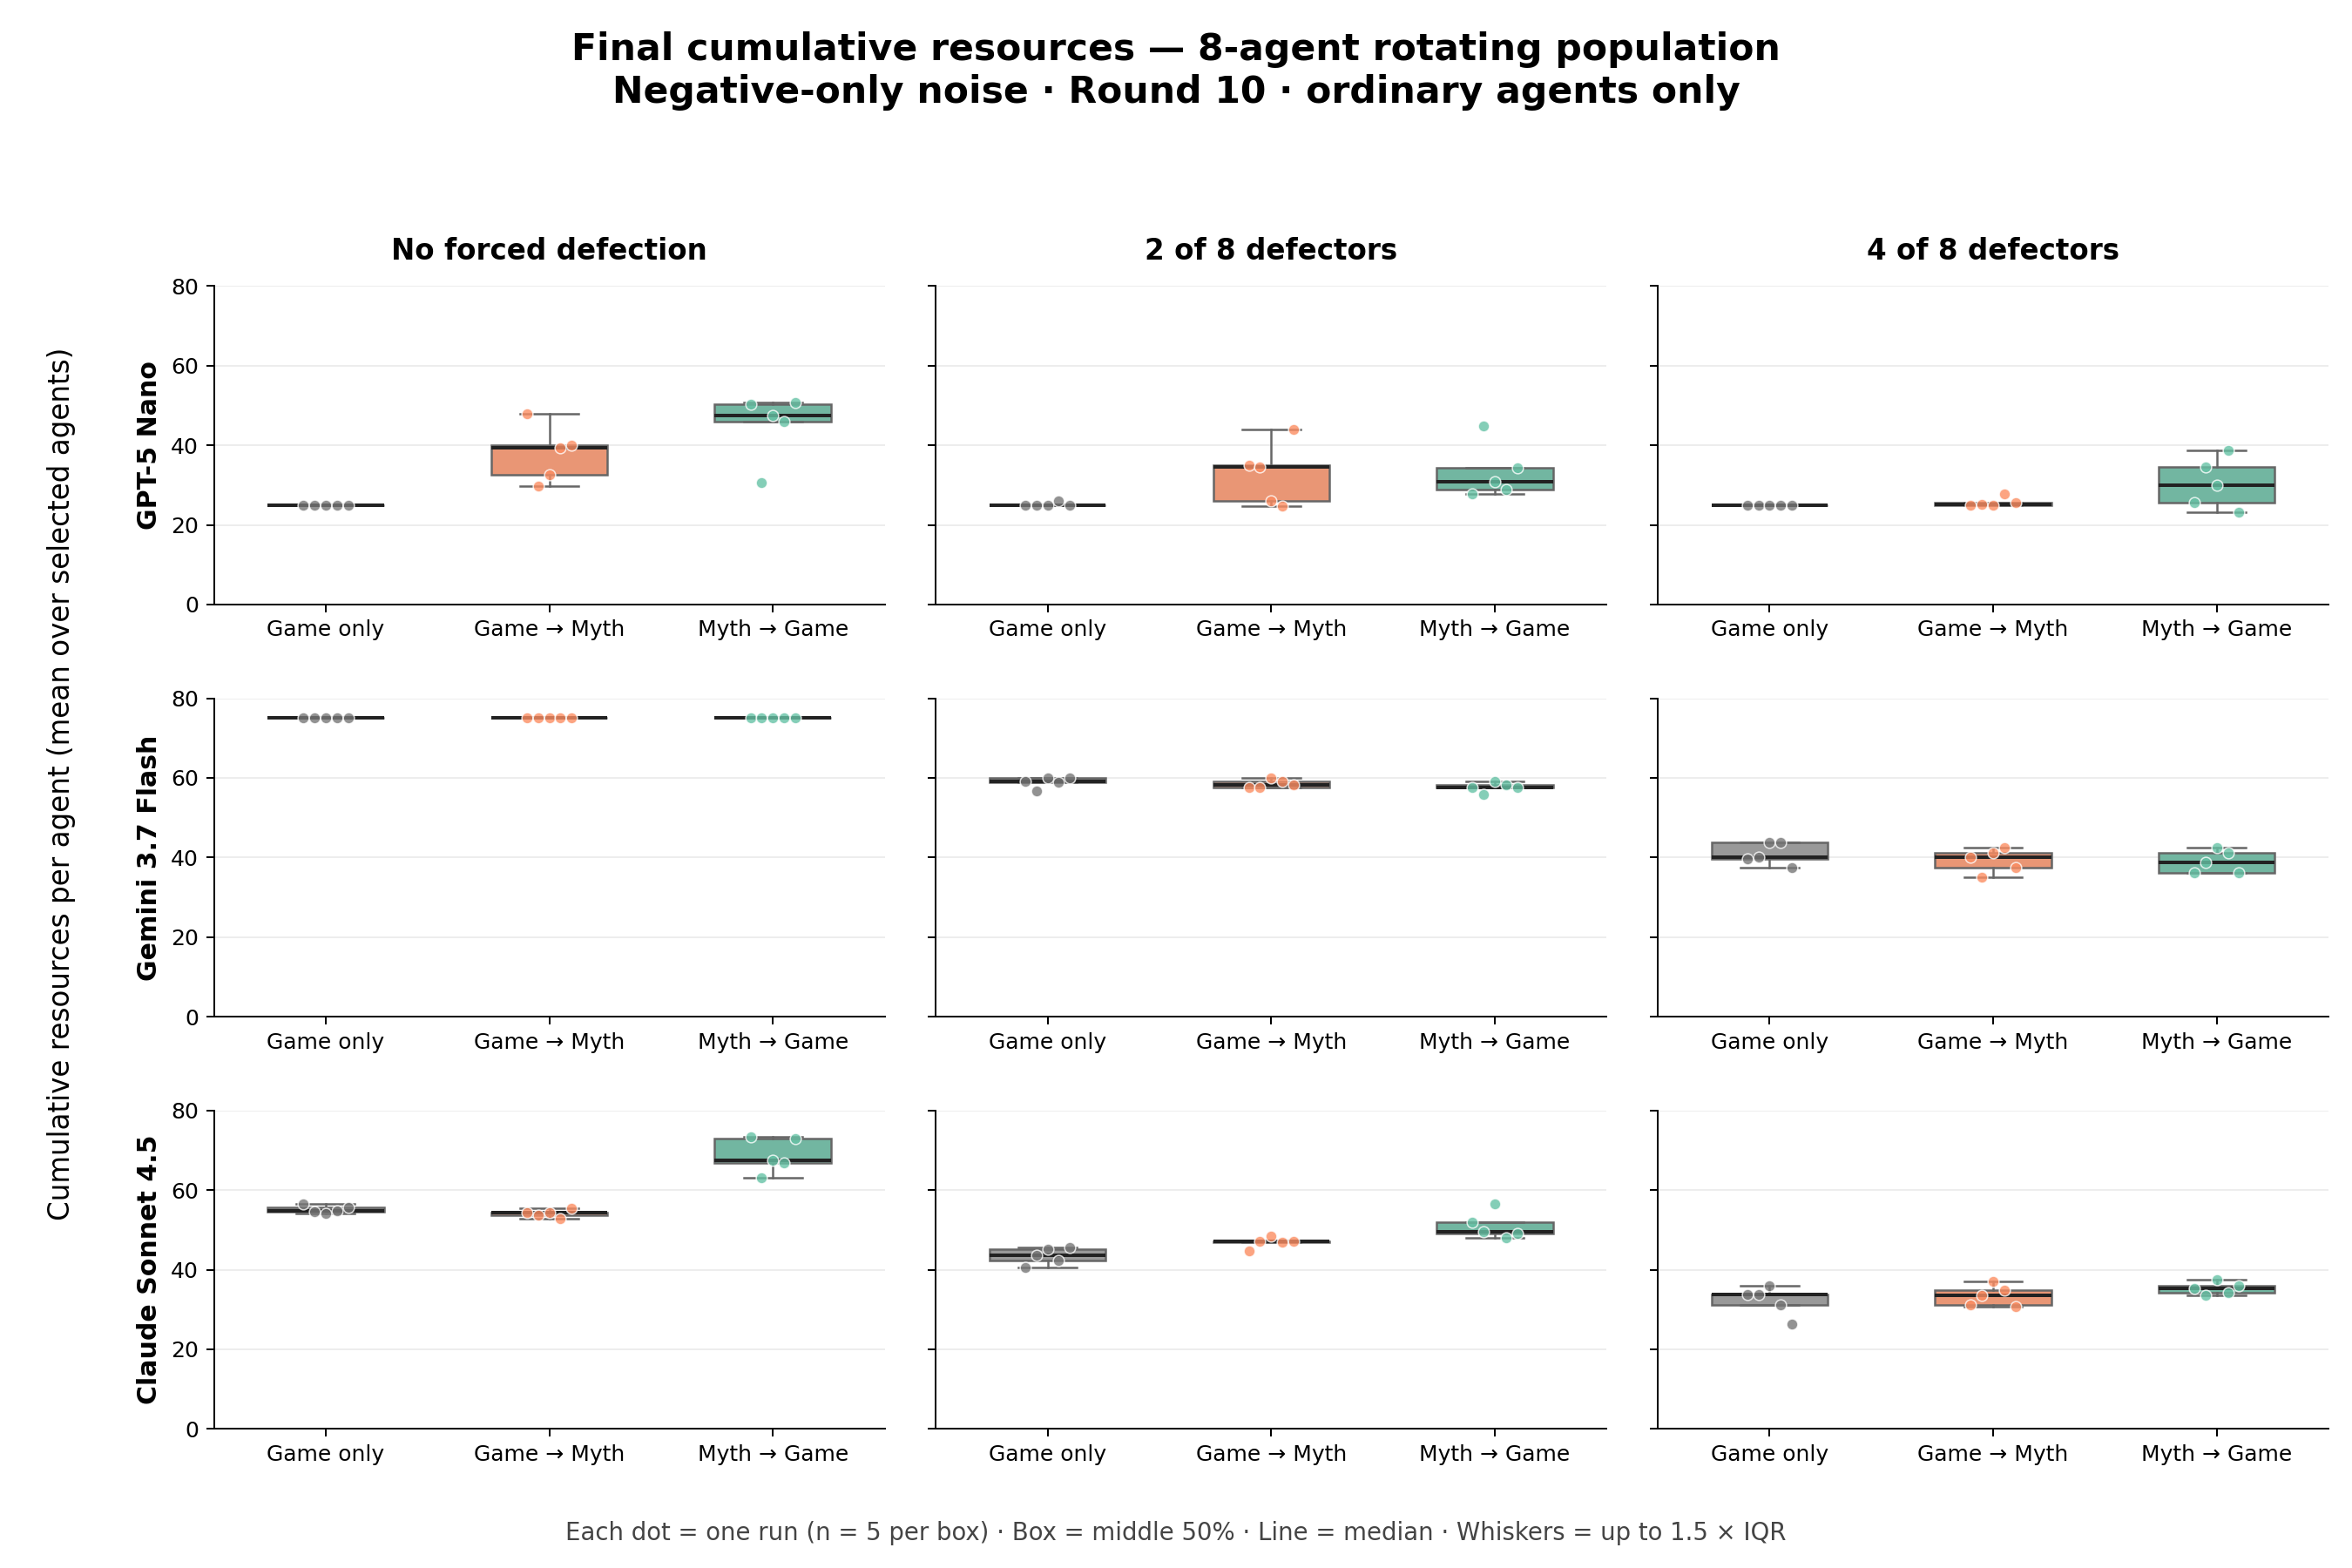
\includegraphics[width=\textwidth]{population_ordinary_agents_boxplots.png}
  \caption{Eight-agent rotating population: final cumulative resources under negative-only noise, averaged over ordinary (non-defector) agents only. Each dot represents one completed run after ten rounds (five runs per condition). Rows show models and columns show forced-defection conditions. Gray denotes Game only, orange Game $\rightarrow$ Myth, and teal Myth $\rightarrow$ Game. Boxes span the interquartile range, the central line marks the median, and whiskers extend to the most extreme observations within 1.5 interquartile ranges of the box. All runs, including outliers, are shown as dots.}
  \label{fig:ordinary-resources-boxplots}
\end{figure*}
 inside the Results section.

\begin{figure*}[tp]
  \centering
  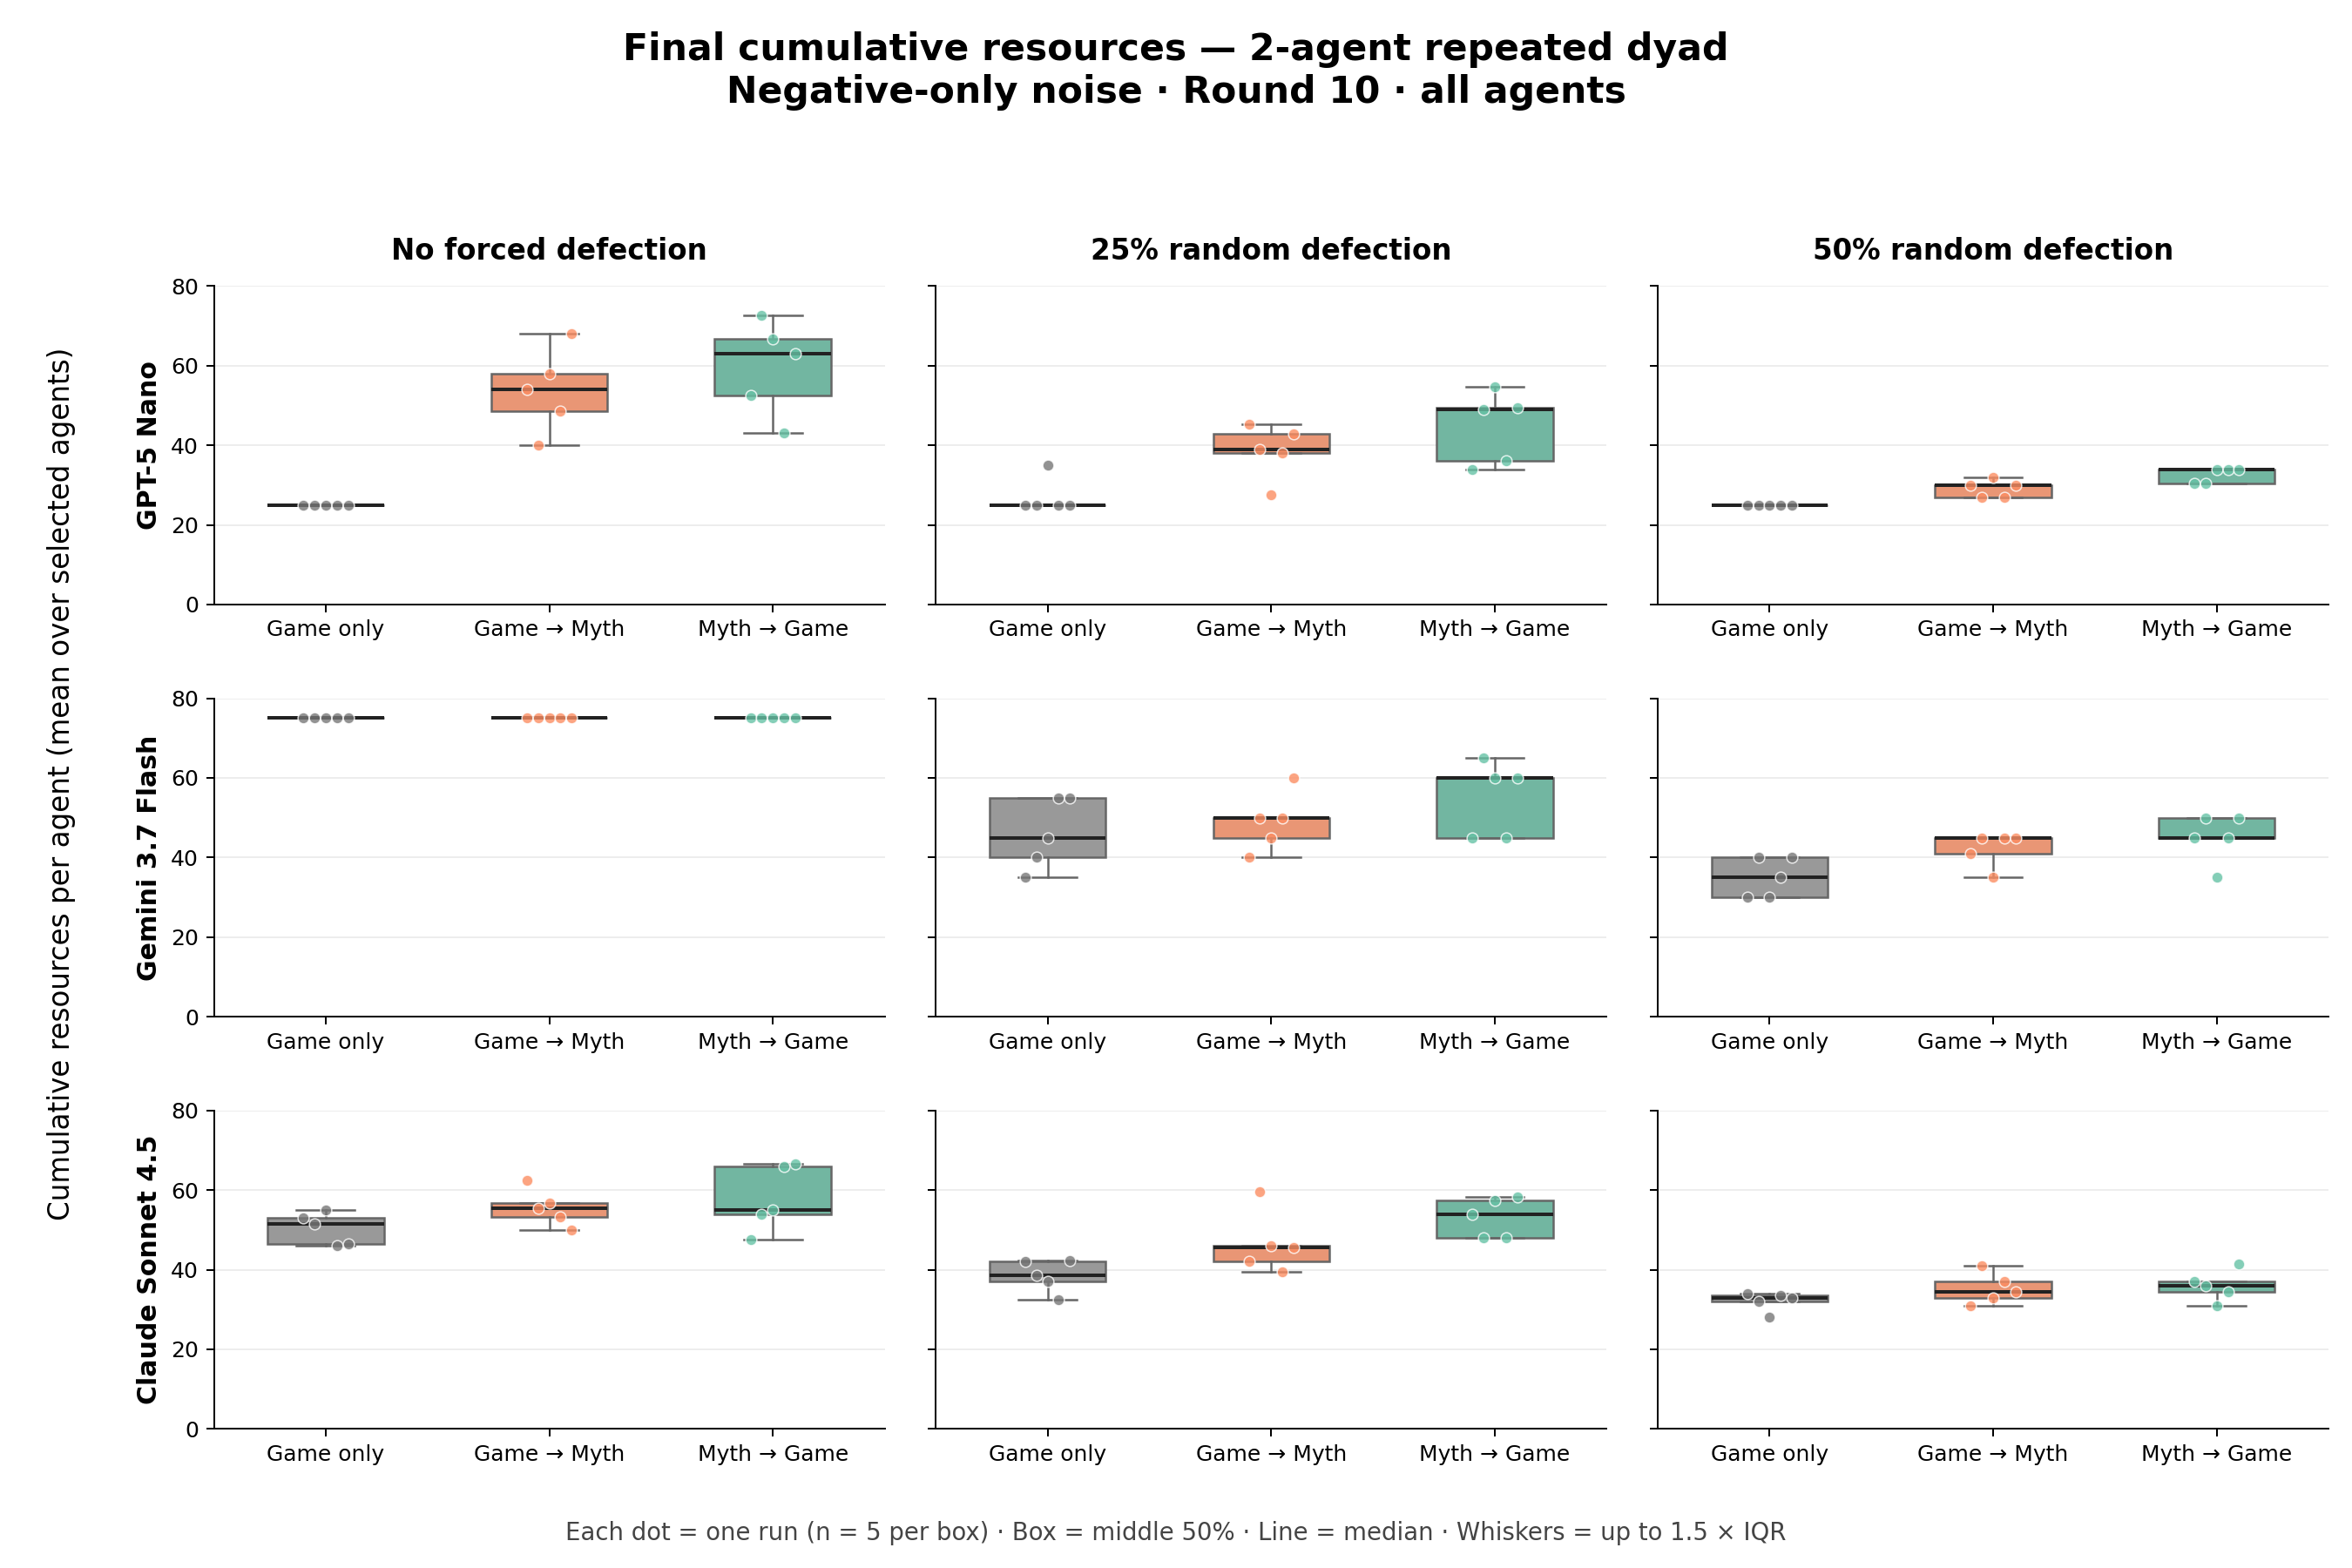
\includegraphics[width=\textwidth]{dyad_all_agents_boxplots.png}
  \caption{Two-agent repeated dyad: final cumulative resources under negative-only noise, averaged over all agents. Each dot represents one completed run after ten rounds (five runs per condition). Rows show models and columns show forced-defection conditions. Gray denotes Game only, orange Game $\rightarrow$ Myth, and teal Myth $\rightarrow$ Game. Boxes span the interquartile range, the central line marks the median, and whiskers extend to the most extreme observations within 1.5 interquartile ranges of the box. All runs, including outliers, are shown as dots.}
  \label{fig:dyad-resources-boxplots}
\end{figure*}

\begin{figure*}[tp]
  \centering
  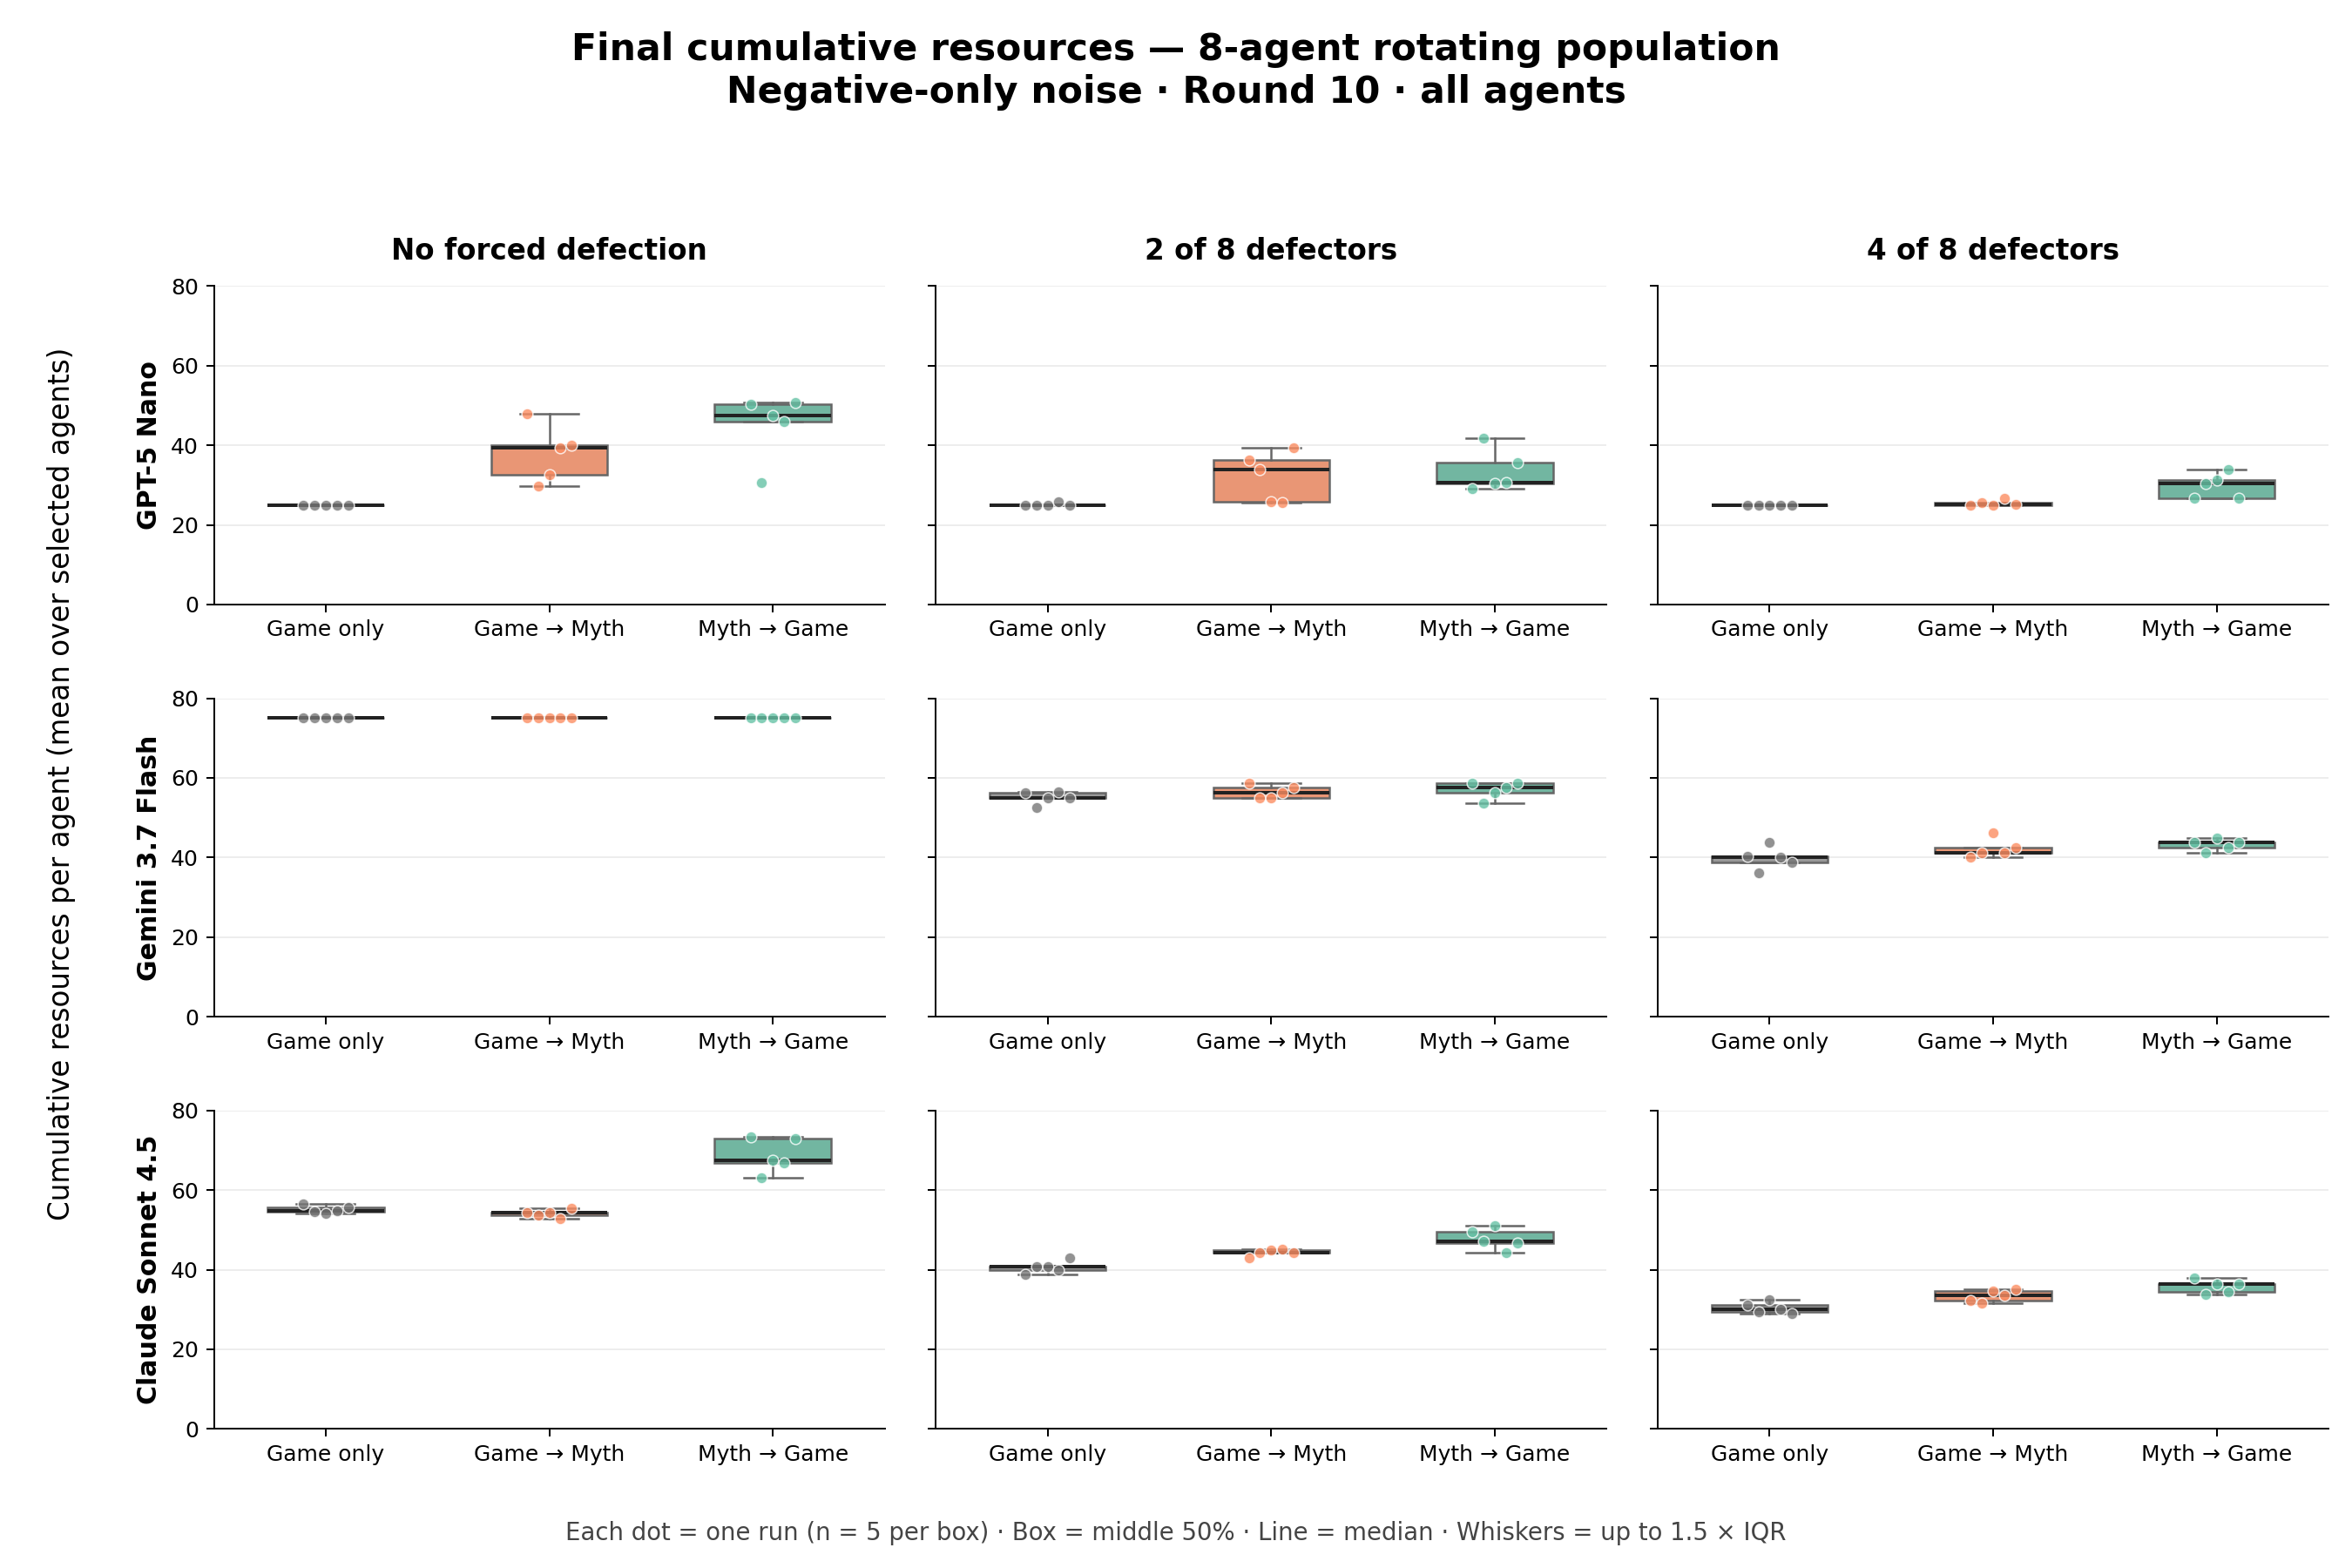
\includegraphics[width=\textwidth]{population_all_agents_boxplots.png}
  \caption{Eight-agent rotating population: final cumulative resources under negative-only noise, averaged over all agents. Each dot represents one completed run after ten rounds (five runs per condition). Rows show models and columns show forced-defection conditions. Gray denotes Game only, orange Game $\rightarrow$ Myth, and teal Myth $\rightarrow$ Game. Boxes span the interquartile range, the central line marks the median, and whiskers extend to the most extreme observations within 1.5 interquartile ranges of the box. All runs, including outliers, are shown as dots.}
  \label{fig:population-resources-boxplots}
\end{figure*}

\begin{figure*}[tp]
  \centering
  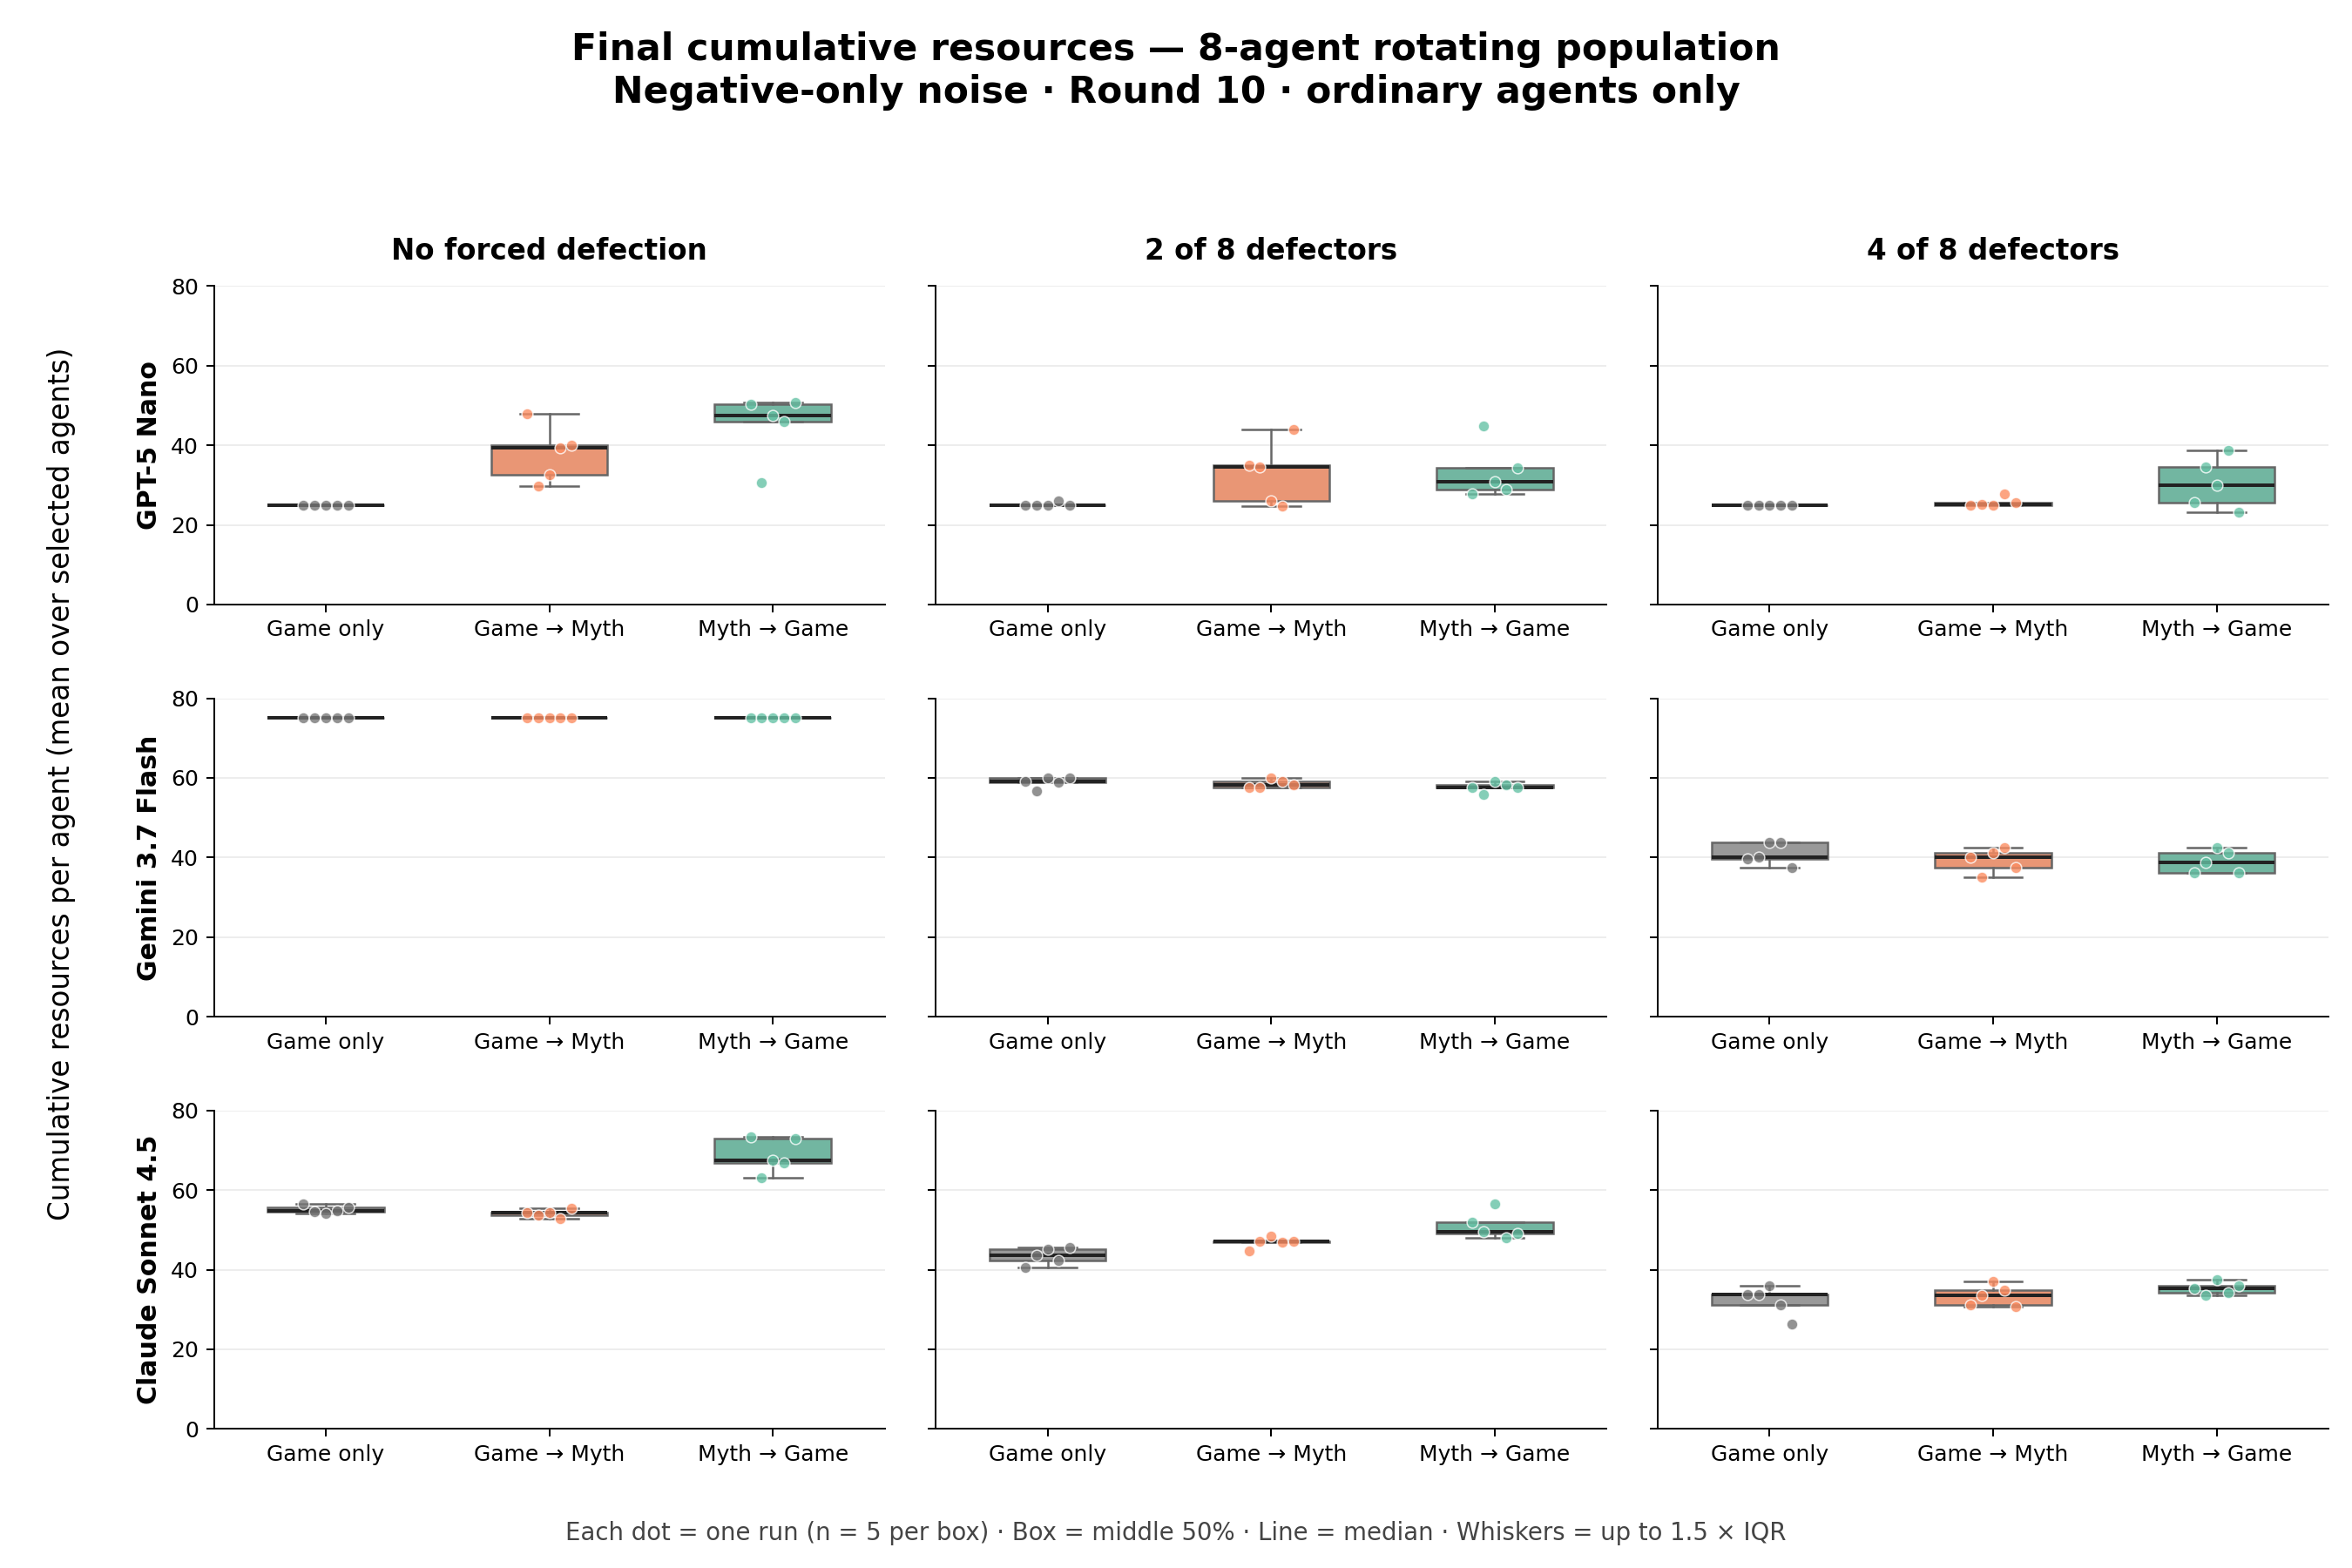
\includegraphics[width=\textwidth]{population_ordinary_agents_boxplots.png}
  \caption{Eight-agent rotating population: final cumulative resources under negative-only noise, averaged over ordinary (non-defector) agents only. Each dot represents one completed run after ten rounds (five runs per condition). Rows show models and columns show forced-defection conditions. Gray denotes Game only, orange Game $\rightarrow$ Myth, and teal Myth $\rightarrow$ Game. Boxes span the interquartile range, the central line marks the median, and whiskers extend to the most extreme observations within 1.5 interquartile ranges of the box. All runs, including outliers, are shown as dots.}
  \label{fig:ordinary-resources-boxplots}
\end{figure*}
